%%%%%%%%%%%%%%%%%%%%%%%%%%%%
%DIF LATEXDIFF DIFFERENCE FILE
%DIF DEL r0.tex                      Tue Apr  7 17:39:20 2015
%DIF ADD Leg_Violence_Named_r1.tex   Tue Apr  7 17:40:09 2015
% Two Sword Lengths Apart
%DIF 3c3
%DIF < % 10 December 2014
%DIF -------
% 7 April 2015 %DIF > 
%DIF -------
%%%%%%%%%%%%%%%%%%%%%%%%%%%%

% !Rnw weave = knitr

\documentclass[a4paper]{article}\usepackage[]{graphicx}\usepackage[]{color}
%% maxwidth is the original width if it is less than linewidth
%% otherwise use linewidth (to make sure the graphics do not exceed the margin)
\makeatletter
\def\maxwidth{ %
  \ifdim\Gin@nat@width>\linewidth
    \linewidth
  \else
    \Gin@nat@width
  \fi
}
\makeatother

\definecolor{fgcolor}{rgb}{0.345, 0.345, 0.345}
\newcommand{\hlnum}[1]{\textcolor[rgb]{0.686,0.059,0.569}{#1}}%
\newcommand{\hlstr}[1]{\textcolor[rgb]{0.192,0.494,0.8}{#1}}%
\newcommand{\hlcom}[1]{\textcolor[rgb]{0.678,0.584,0.686}{\textit{#1}}}%
\newcommand{\hlopt}[1]{\textcolor[rgb]{0,0,0}{#1}}%
\newcommand{\hlstd}[1]{\textcolor[rgb]{0.345,0.345,0.345}{#1}}%
\newcommand{\hlkwa}[1]{\textcolor[rgb]{0.161,0.373,0.58}{\textbf{#1}}}%
\newcommand{\hlkwb}[1]{\textcolor[rgb]{0.69,0.353,0.396}{#1}}%
\newcommand{\hlkwc}[1]{\textcolor[rgb]{0.333,0.667,0.333}{#1}}%
\newcommand{\hlkwd}[1]{\textcolor[rgb]{0.737,0.353,0.396}{\textbf{#1}}}%

\usepackage{framed}
\makeatletter
\newenvironment{kframe}{%
 \def\at@end@of@kframe{}%
 \ifinner\ifhmode%
  \def\at@end@of@kframe{\end{minipage}}%
  \begin{minipage}{\columnwidth}%
 \fi\fi%
 \def\FrameCommand##1{\hskip\@totalleftmargin \hskip-\fboxsep
 \colorbox{shadecolor}{##1}\hskip-\fboxsep
     % There is no \\@totalrightmargin, so:
     \hskip-\linewidth \hskip-\@totalleftmargin \hskip\columnwidth}%
 \MakeFramed {\advance\hsize-\width
   \@totalleftmargin\z@ \linewidth\hsize
   \@setminipage}}%
 {\par\unskip\endMakeFramed%
 \at@end@of@kframe}
\makeatother

\definecolor{shadecolor}{rgb}{.97, .97, .97}
\definecolor{messagecolor}{rgb}{0, 0, 0}
\definecolor{warningcolor}{rgb}{1, 0, 1}
\definecolor{errorcolor}{rgb}{1, 0, 0}
\newenvironment{knitrout}{}{} % an empty environment to be redefined in TeX

\usepackage{alltt}
\usepackage{fullpage}
\usepackage{lscape}
\usepackage[authoryear]{natbib}
\usepackage{setspace}
    \doublespacing
\usepackage{hyperref}
\hypersetup{
    colorlinks,
    citecolor=black,
    filecolor=black,
    linkcolor=cyan,
    urlcolor=cyan
}
\usepackage{booktabs}
\usepackage{dcolumn}
\usepackage{url}
\usepackage{tikz}
\usepackage{todonotes}
\usepackage{verbatim}
\usepackage{endnotes}
\usepackage{graphicx}

%DIF 80a80-82
\usepackage[margins]{trackchanges} %DIF > 
 %DIF > 
\renewcommand*\thetable{\Roman{table}} %DIF > 
%DIF -------
\setlength{\belowcaptionskip}{0.5cm}

%%%%%%% Title Page %%%%%%%%%%%%%%%%%%%%%%%%%%%%%%%%%%%%%%%%%%%%
\title{Two Sword Lengths Apart: Credible Commitment Problems and Physical Violence in \DIFdelbegin \DIFdel{Multi-party Elected }\DIFdelend \DIFaddbegin \DIFadd{Democratic }\DIFaddend National Legislatures}

%DIF 85c88
%DIF < % \author{Christopher Gandrud \\ {\emph{Hertie School of Governance}}\footnote{Post-doctoral Researcher. Friedrichstra{\ss}er 180. 10117 Berlin, Germany. Email: \href{mailto:gandrud@hertie-school.org}{gandrud@hertie-school.org}. Thank you to Gary Cox, Simon Hix, Shirin Rai, Carole Spary, as well as seminar participants at the Hertie School of Governance and Yonsei University for very helpful comments and insights. I would also like to thank Hortense Badarani for excellent research assistance and my students at the LSE for inspiration. Full replication files--including data and source code--can be found at \url{https://github.com/christophergandrud/LegislativeViolence}. An earlier version was circulated under the title ``Two Sword Lengths: Losers' consent and violence in national legislatures''.}}
%DIF -------
%\author{Christopher Gandrud \\ Hertie School of Governance\footnote{Email: \href{mailto:gandrud@hertie-school.org}{gandrud@hertie-school.org}. Thank you to Gary Cox, Simon Hix, Shirin Rai, Carole Spary, as well as seminar participants at the Hertie School of Governance and Yonsei University for very helpful comments and insights. I would also like to thank Hortense Badarani, Tyler Daveron, Alexander Hall, and Lauren Wallace for research assistance, as well as my students at the LSE for inspiration. An earlier version was circulated under the title ``Two Sword Lengths: Losers' consent and violence in national legislatures''.}} %DIF > 
%DIF -------
\IfFileExists{upquote.sty}{\usepackage{upquote}}{}
%DIF PREAMBLE EXTENSION ADDED BY LATEXDIFF
%DIF UNDERLINE PREAMBLE %DIF PREAMBLE
\RequirePackage[normalem]{ulem} %DIF PREAMBLE
\RequirePackage{color}\definecolor{RED}{rgb}{1,0,0}\definecolor{BLUE}{rgb}{0,0,1} %DIF PREAMBLE
\providecommand{\DIFaddtex}[1]{{\protect\color{blue}\uwave{#1}}} %DIF PREAMBLE
\providecommand{\DIFdeltex}[1]{{\protect\color{red}\sout{#1}}}                      %DIF PREAMBLE
%DIF SAFE PREAMBLE %DIF PREAMBLE
\providecommand{\DIFaddbegin}{} %DIF PREAMBLE
\providecommand{\DIFaddend}{} %DIF PREAMBLE
\providecommand{\DIFdelbegin}{} %DIF PREAMBLE
\providecommand{\DIFdelend}{} %DIF PREAMBLE
%DIF FLOATSAFE PREAMBLE %DIF PREAMBLE
\providecommand{\DIFaddFL}[1]{\DIFadd{#1}} %DIF PREAMBLE
\providecommand{\DIFdelFL}[1]{\DIFdel{#1}} %DIF PREAMBLE
\providecommand{\DIFaddbeginFL}{} %DIF PREAMBLE
\providecommand{\DIFaddendFL}{} %DIF PREAMBLE
\providecommand{\DIFdelbeginFL}{} %DIF PREAMBLE
\providecommand{\DIFdelendFL}{} %DIF PREAMBLE
%DIF END PREAMBLE EXTENSION ADDED BY LATEXDIFF
%DIF PREAMBLE EXTENSION ADDED BY LATEXDIFF
%DIF HYPERREF PREAMBLE %DIF PREAMBLE
\providecommand{\DIFadd}[1]{\texorpdfstring{\DIFaddtex{#1}}{#1}} %DIF PREAMBLE
\providecommand{\DIFdel}[1]{\texorpdfstring{\DIFdeltex{#1}}{}} %DIF PREAMBLE
%DIF END PREAMBLE EXTENSION ADDED BY LATEXDIFF

\begin{document}

\maketitle

\DIFaddbegin \begin{center}
\DIFadd{Word Count: 11,352
}\end{center}

\DIFaddend %%%%%%% Abstract %%%%%%%%%%%%%%%%%%%%%%%%%%%%%%%%%%%%%%%%%%%%
\begin{abstract}
\DIFdelbegin \DIFdel{Multi-party elected }\DIFdelend \DIFaddbegin \DIFadd{Ideally, democratic }\DIFaddend national legislatures should be venues for peacefully resolving conflicts between opposing groups. However, they can become scenes of physical violence. Such violence is an indication that a country's legislative institutions are functioning far from perfectly as legislative actors are deciding to disregard the rules of the game. In some cases, such as \DIFdelbegin \DIFdel{recently in Ukraine }\DIFdelend \DIFaddbegin \DIFadd{in Ukraine throughout the early 2000s}\DIFaddend , violence can indicate and possibly fuel deeper political divisions. In this first global study of legislative violence, I show that brawls are more likely when legislators find it difficult to credibly commit to follow peaceful bargains. Credible commitment problems are more acute in countries with disproportionate electoral \DIFdelbegin \DIFdel{outcomes and }\DIFdelend \DIFaddbegin \DIFadd{outcomes--i.e. when votes for parties do not closely correspond to the legislative seats they are given--and }\DIFaddend in new democracies. I find robust evidence for this argument using a case study of legislative violence in the antebellum United States Senate and a new global data set. \DIFaddbegin \DIFadd{In addition I find evidence that violence is more likely in legislatures with small minority governments.
}\DIFaddend \end{abstract}


\paragraph{Keywords:} legislatures, violence, credible commitment problems, electoral proportionality, institutional design, majority and minority governments

\vspace{0.3cm}

%%%%%%% Introduction %%%%%%%%%%%%%%%%%%%%%%%%%%%%%%%%%%%%%%%%%%%%

Though legislators in democracies are often described as `battling' or `fighting' we expect these battles to be in terms of rhetoric and procedural manoeuvres, circumscribed by non-violent rules, that culminate in votes. The outcomes of these contests are then respected by all legislators. However, metaphorical battles sometimes become physical fights between \DIFdelbegin \DIFdel{members of legislatures}\DIFdelend \DIFaddbegin \DIFadd{legislators}\DIFaddend .

Many \DIFdelbegin \DIFdel{legislatures}\DIFdelend \DIFaddbegin \DIFadd{parliaments}\DIFaddend ' histories contain incidents of physical violence between legislators. In 1856 a member of the United States House of Representatives caned a senator unconscious in the Senate chamber \citep{USSenateCanning}. It has been suggested that the United Kingdom's House of Commons is physically designed to prevent violence between members. The Government and Opposition benches are said to be ``two sword lengths apart" \citep{ParliamentUKSword} so that duels will be fought with words rather than swords\DIFdelbegin \DIFdel{. Actual, }\DIFdelend \DIFaddbegin \DIFadd{, a central democratic ideal \mbox{%DIFAUXCMD
\cite[220]{Schwarzmantel2010}
}%DIFAUXCMD
. Actual }\DIFaddend sword fights do not seem to have taken place in the Commons chamber, but violent incidences did occur in the 1800s \DIFdelbegin \DIFdel{\mbox{%DIFAUXCMD
\citep[see][]{ByrneViolence}
}%DIFAUXCMD
}\DIFdelend \DIFaddbegin \DIFadd{\mbox{%DIFAUXCMD
\citep[]{ByrneViolence}
}%DIFAUXCMD
}\DIFaddend . Violence in legislatures continues to occur. Recent instances of violence between legislators include brawls in South Korea in 2009\footnote{See \url{http://dailym.ai/1rHLruX}. Accessed October 2014} and in Ukraine during the years leading up to the civil war.\footnote{For example see \url{http://online.wsj.com/articles/SB10001424052748704471204575209572380473814}. Accessed October 2014} In 2013 a large confrontation happened in the Venezuelan National Assembly when the Assembly President withheld speaking time from legislators who did not recognize president's victory \DIFdelbegin \DIFdel{in a very }\DIFdelend \DIFaddbegin \DIFadd{after a }\DIFaddend highly contested election.\footnote{See \url{http://edition.cnn.com/2013/04/30/world/americas/venezuela-lawmakers-violence/index.html}. Accessed October 2014.}

Physical violence is a dramatic break from scholars' assumption that compliance with legislative rules of the game is a given and as such \DIFdelbegin \DIFdel{symbolizes poorly functioning }\DIFdelend \DIFaddbegin \DIFadd{can symbolize poorly functioning democratic }\DIFaddend legislative institutions. Some work has examined the strategic and expressive choices politicians make when they decide not to participate in the democratic rules of the game\DIFaddbegin \DIFadd{, including before elections }\DIFaddend \citep{wilkinson2006,Beaulieu2008,BeaulieuForthcoming}. In this \DIFdelbegin \DIFdel{paper }\DIFdelend \DIFaddbegin \DIFadd{article }\DIFaddend I extend this work by advancing a theory of legislative violence in \DIFdelbegin \DIFdel{multi-party elected }\DIFdelend \DIFaddbegin \DIFadd{democratic }\DIFaddend national legislatures and test it using both case study and global-level data. Indeed, this \DIFdelbegin \DIFdel{paper }\DIFdelend \DIFaddbegin \DIFadd{article }\DIFaddend includes the first cross-country description of violence between legislators. It also provides us with an important window for understanding what makes legislatures work (or not) as institutions for peacefully resolving disputes between opposing parties.\footnote{Note that the underlying process I discuss that creates conditions for violence likely also creates environments where legislators use other types of less violent--and less easily observable on a global scale--forms of legislative rule breaking.}

I begin the \DIFdelbegin \DIFdel{paper }\DIFdelend \DIFaddbegin \DIFadd{article }\DIFaddend by advancing an argument for understanding when legislative violence between members of \DIFdelbegin \DIFdel{multi-party }\DIFdelend \DIFaddbegin \DIFadd{democratic }\DIFaddend elected legislatures is more likely. Though legislators' personalities surely play some part in any given violent incident, I argue that the probability of violence is strongly influenced by the wider political environment. In particular, violence is much more likely when there are \emph{credible commitment problems} that incentivize legislators to break peaceful bargains. At least two observable \DIFdelbegin \DIFdel{institutional }\DIFdelend factors are important for affecting the likelihood that commitments will be adhered to: the \emph{proportionality of \DIFdelbegin \DIFdel{a country's }\DIFdelend electoral outcomes}\DIFdelbegin \DIFdel{and the }\DIFdelend \DIFaddbegin \DIFadd{--e.g. when votes for parties do not closely correspond to the legislative seats they are given--and the }\DIFaddend \emph{age of \DIFdelbegin \DIFdel{its }\DIFdelend democracy}. After proposing this argument and discussing a number of key alternative explanations, I begin to empirically examine it with a case study of violence in the antebellum United States Senate. I then move to \DIFdelbegin \DIFdel{a global level }\DIFdelend \DIFaddbegin \DIFadd{the core of the empirical analysis: a global-level }\DIFaddend study of contemporary legislative violence by describing a new data set of legislative violence. In this section\DIFaddbegin \DIFadd{, }\DIFaddend I also demonstrate simple associations between my argument's key variables and violence on a global scale. I then discuss the variables and parametric regression models I use to further study these events. Finally, I lay out the evidence from these models that legislative violence is more prevalent in countries with disproportionate electoral outcomes and in new democracies. I also find that violence is more likely in legislatures with small minority governments. I conclude the \DIFdelbegin \DIFdel{paper }\DIFdelend \DIFaddbegin \DIFadd{article }\DIFaddend with a discussion of the possible implications of these findings for democratic institution designers and directions for future research.

%%%%%%%%%%%%%%%%%%%%%%%%%%%%%%%%%%%%%%%%%%%%%% Previous Research & Framework

\DIFdelbegin \section{\DIFdel{Understanding Legislative Violence}}
%DIFAUXCMD
\addtocounter{section}{-1}%DIFAUXCMD
\DIFdelend \DIFaddbegin \section*{\DIFadd{Understanding Legislative Violence}}
\DIFaddend 

Legislative violence, like other forms of violent disruption \DIFdelbegin \DIFdel{\mbox{%DIFAUXCMD
\citep[see][]{Beaulieu2008,BeaulieuForthcoming,wilkinson2006}
}%DIFAUXCMD
}\DIFdelend \DIFaddbegin \DIFadd{\mbox{%DIFAUXCMD
\citep[]{Beaulieu2008,BeaulieuForthcoming,wilkinson2006}
}%DIFAUXCMD
}\DIFaddend , could be used for strategic purposes by both legislative winners and losers. Legislative losers--those who are not in control of the ``legislative cartel''  that sets the agenda \citep{cox2007} and \DIFaddbegin \DIFadd{so }\DIFaddend are not part of the \DIFdelbegin \DIFdel{deciding majority--may }\DIFdelend \DIFaddbegin \DIFadd{group that passes controls legislative outcomes}\footnote{\DIFadd{There is strong evidence that those who control the legislative agenda tend to control what bills are brought up for a vote and in turn what bills are passed \mbox{%DIFAUXCMD
\citep[93]{tsebelis2002}
}%DIFAUXCMD
.}}\DIFadd{--may }\DIFaddend use violence to stall legislation or rule changes they dislike. Winners--those in the legislative cartel--could use violence to prevent losers from utilizing procedures that might constrain their \DIFdelbegin \DIFdel{decision-making power }\DIFdelend \DIFaddbegin \DIFadd{power to control the legislative agenda and therefore legislative policy outcomes}\DIFaddend . Both winners and losers may use violence to shore up support among their proponents, as a way of expressing dissatisfaction with legislative outcomes, and to publicize issues they and their supporters care about \DIFaddbegin \DIFadd{\mbox{%DIFAUXCMD
\citep{Spary2013}
}%DIFAUXCMD
}\DIFaddend . Winners may not only use active violence, but also might make a strategic choice not to use their powers, e.g. control of security forces, to prevent or curtail losers' violence with the hope that losers will be publicly discredited.\DIFaddbegin \footnote{\DIFadd{Examining the interactions of both those in power and those out of it is in contrast to important strains in the political protest movement literature. Political opportunity structure theories of protest have examined how, largely exogenous, state power \mbox{%DIFAUXCMD
\citep{skocpol1979}
}%DIFAUXCMD
and state receptiveness to protester demand \mbox{%DIFAUXCMD
\citep{mcadam1982,tarrow1989}
}%DIFAUXCMD
encourage or discourage protest. In my approach, winners clearly play an important role in causing violence, they may even be violent. However, I do not treat them as exogenous. They are goal-seeking actors engaged in bargaining with other legislators.}}
\DIFaddend 

Just because actors can gain a strategic advantage or express their discontent through violence does not mean they will choose to. Though violence may have strategic benefits, it also entails costs. Violent conflict has physical costs. In a number of incidents legislators have been hospitalized or even, as in the case of Charles Sumner discussed below, almost died. Beyond the physical costs of legislative violence, there may be other costs such as legal penalties and reputational \DIFdelbegin \DIFdel{costs}\DIFdelend \DIFaddbegin \DIFadd{damage}\DIFaddend .

However, there are situations where legislators perceive the benefits of violence to be greater than the costs. Violence in \DIFdelbegin \DIFdel{multi-party elected }\DIFdelend \DIFaddbegin \DIFadd{democratic }\DIFaddend legislatures is often precipitated by situations where legislators find it difficult to credibly commit to follow peaceful bargaining outcomes. In these situations the perceived benefits of violence can outweigh the costs. \DIFaddbegin \DIFadd{Violence becomes bargaining by other means. }\DIFaddend \cite{Fearon1995} argued that when actors are not able to make credible commitments the benefits from violent conflict can outweigh the costs making violence more likely \cite[see also][]{Powell2006}. If it is difficult to believe that a peaceful bargaining outcome will actually happen because bargained commitments will likely be broken, actors will choose violence to achieve their goals. This logic is applicable to legislatures. In \DIFdelbegin \DIFdel{multi-party elected }\DIFdelend \DIFaddbegin \DIFadd{democratic }\DIFaddend legislatures winners and losers--who may some day become winners--need to be able to credibly commit to not use or remake legislative procedures in their narrow self-interest. They need to commit to limits on their power \citep{riker1982,Gaubatz1996}, especially legislative rules and procedures that are the result of peaceful bargaining processes. If \DIFdelbegin \DIFdel{they are not able to credibly make these commitments }\DIFdelend \DIFaddbegin \DIFadd{these credible commitments are not possible }\DIFaddend then legislators may come to believe that disruption and violence is the best way to achieve their \DIFaddbegin \DIFadd{legislative, including policy }\DIFaddend goals, despite its costs. What makes legislative credible commitment problems more or less severe?

\DIFaddbegin \subsection*{\DIFadd{Observing Situations Where Credible Commitment Problems are Worse}}

\DIFadd{To empirically test my theory I focus on two clearly observable institutional factors that structure bargaining by influencing legislators' credible commitment problems: proportionality of electoral outcomes and age of democracy. Please note that these are likely not the only factors that shape credible commitments, but they are definitively observable in a cross-country study.
}

\paragraph{\DIFadd{Proportional Electoral Outcomes}}

\DIFaddend Credible commitment problems are generally smaller and therefore violence is less likely \DIFdelbegin \DIFdel{when }\DIFdelend \emph{\DIFaddbegin \DIFadd{when }\DIFaddend seats in the legislature and legislative resources \DIFaddbegin \DIFadd{more generally}\DIFaddend , such as speaking time and committee appointments, proportionally correspond to voters' support}. \DIFdelbegin \DIFdel{For simplicity I will refer to such legislatures as `fair'}\DIFdelend \DIFaddbegin \DIFadd{Control over seats and other legislative resources such as the agenda often directly corresponds to what bills pass the legislature}\DIFaddend . I argue that a lack of correspondence between legislative power and voter support increases legislative credible commitment problems in at least two ways: it (a) creates possibilities for shifts in power from those who benefit from the status quo to beneficiaries of \DIFdelbegin \DIFdel{fairer rules }\DIFdelend \DIFaddbegin \DIFadd{rules that would more closely align legislative resources with voter support }\DIFaddend and (b) prevents fairness equilibria.

\DIFdelbegin \DIFdel{Unfair }\DIFdelend \DIFaddbegin \DIFadd{Disporoportionate }\DIFaddend legislatures have the possibility for large and rapid shifts in legislative power from those who benefit from the status quo rules to those \DIFdelbegin \DIFdel{that }\DIFdelend \DIFaddbegin \DIFadd{who }\DIFaddend would benefit from new rules. For example, if an electoral system that creates disproportionate outcomes becomes more proportional, then the winning parties may be likely to change over the course of one election. The new winners could then further alter legislative procedures \DIFaddbegin \DIFadd{and legislative outcomes }\DIFaddend to benefit themselves through control of the legislative \DIFdelbegin \DIFdel{cartel}\DIFdelend \DIFaddbegin \DIFadd{agenda}\DIFaddend . \cite{Powell2004,Powell2006} identified major commitment problems in bargains over issues affecting future bargaining power when there could be large and rapid power shifts. We can apply his logic to legislatures. Temporarily weak legislators--those with disproportionately fewer seats and access to legislative resources under the status quo--who are not in the legislative cartel need to `buy off' those that are temporarily strong--the beneficiaries of the status quo in the cartel--in order to avoid the strong changing the rules to further benefit themselves. `Buying off' in this context may simply mean agreeing to continue rules that \DIFdelbegin \DIFdel{make the legislature unfair }\DIFdelend \DIFaddbegin \DIFadd{distribute legislative resources away from electoral support }\DIFaddend at the status quo level. However, because the presently weak have the potential to be much stronger, they are likely to renege on agreements that disproportionately benefit the temporarily strong. \DIFdelbegin \DIFdel{They }\DIFdelend \DIFaddbegin \DIFadd{The temporarily strong }\DIFaddend may also have an \DIFdelbegin \DIFdel{incentive }\DIFdelend \DIFaddbegin \DIFadd{incentives }\DIFaddend to use disruption or violence to prevent further rule changes that limit their power or indeed force the rules to \DIFdelbegin \DIFdel{become fairer to actively increase }\DIFdelend \DIFaddbegin \DIFadd{distribute resources such that it actively increases }\DIFaddend their power. Importantly, in the absence of credible commitments from the temporarily weak, the \emph{temporarily strong may use preemptive violence to prevent \DIFaddbegin \DIFadd{changes to }\DIFaddend the rules \DIFdelbegin \DIFdel{from becoming fairer}\DIFdelend \DIFaddbegin \DIFadd{that distribute legislative resources in closer alignment with electoral support}\DIFaddend }.

Why do \DIFdelbegin \DIFdel{very fair legislatures }\DIFdelend \DIFaddbegin \DIFadd{legislatures that have a close correspondence between legislative resources and voter support }\DIFaddend not create equally large credible commitment problems? Presumably legislators that would benefit from \DIFdelbegin \DIFdel{a large increases in unfairness }\DIFdelend \DIFaddbegin \DIFadd{legislative resources being unmoored from voter support }\DIFaddend would find it difficult to credibly commit. In other words, why would a \DIFdelbegin \DIFdel{fair legislature }\DIFdelend \DIFaddbegin \DIFadd{legislature where resources were distributed closely according to electoral support }\DIFaddend create an equilibrium? Rabin's \citeyearpar{Rabin1993} work studying bargaining consequences when actors care about fairness in addition to material well-being provides an answer. Because actors care about \DIFdelbegin \DIFdel{fairness}\DIFdelend \DIFaddbegin \DIFadd{``fair''}\DIFaddend , they are more likely to maintain commitments (punish defectors), even if it hurts their material well-being, when others are being fair (unfair). One form of punishment could be reputational damage inflicted in \DIFdelbegin \DIFdel{fair }\DIFdelend \DIFaddbegin \DIFadd{proportional }\DIFaddend systems by both supporters and opponents of violent legislators who care about fairness. This reduces legislators' incentives to defect from fair rules and bargains even if they could gain legislative power by increasing unfairness. As such credible commitment problems are lower and actors can reach a ``fairness equilibrium''. Experimental research supports the idea that commitments are more credible if they are fairer \citep{Ellingsen2004} and can even act as an enforcement device for incomplete contracts \DIFdelbegin \DIFdel{\mbox{%DIFAUXCMD
\citep[see][for a review]{Fehr2008}
}%DIFAUXCMD
}\DIFdelend \DIFaddbegin \DIFadd{\mbox{%DIFAUXCMD
\citep{Fehr2008}
}%DIFAUXCMD
}\DIFaddend .

\DIFdelbegin \subsection{\DIFdel{Observing Situations Where Credible Commitment Problems are Worse}}
%DIFAUXCMD
\addtocounter{subsection}{-1}%DIFAUXCMD
%DIFDELCMD < 

%DIFDELCMD < %%%
\DIFdel{To empirically test my theory I focus on two clearly observable institutional factors that structure bargaining by influencing legislators' credible commitment problems: proportionality of electoral outcomes and age of democracy. Please note that these are likely not the only factors that shape credible commitments, but they are definitively observable in a cross-country study.
}%DIFDELCMD < 

%DIFDELCMD < %%%
\paragraph{\DIFdel{Proportional Electoral Outcomes}}
%DIFAUXCMD
\addtocounter{paragraph}{-1}%DIFAUXCMD
%DIFDELCMD < 

%DIFDELCMD < %%%
\DIFdel{Possibly the most important and clearly observable component of legislature fairness is the proportionality of the election that allocated its seats and therefore the control of its procedures. Disproportional, i.e. unfair, electoral outcomes create credible commitment problems as they create the potential for shifts in power from beneficiaries of unfair to fair rules. More proportional systems conversely enable fairness equilibria. }\DIFdelend At what observable levels of disproportionately would we expect to \DIFdelbegin \DIFdel{see }\DIFdelend \DIFaddbegin \DIFadd{empirically observe }\DIFaddend more violence? At most levels of disproportionately there may be credible commitment problems to some degree, because there will be legislators who benefit from an increase in proportionality. It is only when outcomes are close to perfectly proportional that the gains from increasing proportionality are very small or virtually none existent. At the same time in systems with very proportional electoral outcomes it is \DIFdelbegin \DIFdel{easy for all to }\DIFdelend \DIFaddbegin \DIFadd{more likely that all sides }\DIFaddend identify the electoral outcomes as fair, thus enabling fairness equilibria.\footnote{When there is ambiguity over how fair the system is actors may not impose very high costs, such as reputational damage, for breaking the rules.} Because of this we should not expect a linear relationship between disproportionately and violence. There should instead be a threshold effect where very proportional electoral outcomes will have very low levels of violence due to very small or non-existent credible commitment problems.

Recent empirical research on the functional form of the relationship between political trust and disproportionality provides some initial evidence for the claim that there could be a threshold effect between disproportionality and legislative violence. \cite{Marien2011} found that there was a curvilinear relationship between proportional electoral outcomes and citizens' political trust. Feelings of political trust were highest with very proportional outcomes as well as disproportional or majoritarian systems. Countries in the middle had the lowest trust. Marien argues that high trust in very proportional systems is caused by high fairness. The fairness effect seems to quickly disappear as we move in the direction of more disproportionate outcomes. Marien argues that high voter trust in very disproportionate countries is caused not by fairness, but by high accountability. So should we expect a similar curvilinear relationship between proportionality and legislative violence? Probably not. Though accountability may please voters in general, there is little reason to believe that this will ameliorate the credible commitment problems among legislators created by unfairness. \DIFdelbegin %DIFDELCMD < 

%DIFDELCMD < %%%
\DIFdelend For these reasons \DIFdelbegin \emph{\DIFdel{we should expect countries with very proportional outcomes to have lower incidences of violence. All other countries should be more likely to have more violence.}}
%DIFAUXCMD
\DIFdelend \DIFaddbegin \DIFadd{we should expect:
}\DIFaddend 

\DIFaddbegin \begin{quote}
    \DIFadd{H1: }\emph{\DIFadd{Countries with very proportional outcomes to have lower incidences of violence. All other countries should be more likely to have more violence.}}
\end{quote}

\DIFaddend It's important to note that though the exact type of electoral system is ultimately interesting to us from an institutional design point of view, we should not confuse ``the outcome of an electoral system with its mechanics'' \citep[][109]{Golder2005}. When studying legislative fairness and credible commitment problems we are more interested in how proportional electoral outcomes are, rather than the exact type of electoral system that produced these outcomes.

\paragraph{New vs. Old Democracies}

Legislators in older democracies are more likely to \DIFdelbegin \DIFdel{view their parliament as fair and }\DIFdelend \DIFaddbegin \DIFadd{have good information about the likelihood that currently ruling parties will actually adhere to their commitments. As such they }\DIFaddend are more likely to be able to make \DIFaddbegin \DIFadd{new }\DIFaddend credible commitments. There are a number of reasons for this. In new democracies, as with political regime change in general, the rules of the game are in flux and have not been fully institutionalized. This can give present winners considerable power to set the rules to their advantage. The first actors to gain power after a transition--whose decision-making power may be disproportionately large compared to their electoral support--may be better able to establish \DIFdelbegin \DIFdel{unfair rules , entrenching their power }\DIFdelend \DIFaddbegin \DIFadd{rules and policies, that entrench their power and disadvantage others in the future }\DIFaddend \cite[108]{Saideman2002}. This could lead to credible commitment problems between the temporarily strong that are making the rules during the democratic transition and the temporarily weak who could gain more if the rules \DIFdelbegin \DIFdel{were fairer}\DIFdelend \DIFaddbegin \DIFadd{more proportionally distributed resources}\DIFaddend .

Also, in the relatively early days of a democracy the legislative party system may be shifting considerably \DIFdelbegin \DIFdel{\mbox{%DIFAUXCMD
\cite[see][161 for a review]{Mainwaring2007b}
}%DIFAUXCMD
}\DIFdelend \DIFaddbegin \DIFadd{\mbox{%DIFAUXCMD
\cite[161]{Mainwaring2007b}
}%DIFAUXCMD
}\DIFaddend , possibly as politicians work out electoral coordination problems \citep{cox1997}. New democracies may also have rapidly changing economies and \DIFaddbegin \DIFadd{possibly }\DIFaddend demographics that further change the party system and the proportionality of legislative rules. Even if rules \DIFdelbegin \DIFdel{were fair }\DIFdelend \DIFaddbegin \DIFadd{proportionally distributed resources }\DIFaddend when they were created, they may quickly become less so as the country changes. On average, these shifts could be much larger in new as opposed to old democracies. As we will see in the antebellum US case below, large rapid demographic and party system shifts dramatically altered the fairness of the distribution of power in the US Senate between pro and anti-slavery senators around the 1840s and 1850s. Because of the instability of new party systems, there is a greater likelihood that legislatures could become unfair leading to credible commitment problems and violence.

The alternation of power that generally occurs as democratic regimes survive longer gives legislators more information about the credibility of others' commitments. In new democracies actors simply may not have gathered enough information to know if they can someday become winners. Losers in new democracies may not have learned that ``pretenders to office can expect to reach it, losers can expect to come back'' \citep[][36]{Przeworski1991}. Actual alternations of power allow legislators to gather better information about the credibility of commitments to allow fair alternations of power. Increased information about others' abilities to make credible commitments could strengthen the credibility of future commitments, thus reducing violence.

There may also be a survivor bias created as democracies age. If legislatures are unable to overcome credible commitment problems in some way, legislative institutions will not peacefully organize bargaining. This could lead to discontent and social unrest both inside and outside of the legislature, possibly resulting in democratic collapse. New democracies unable to overcome credible commitment problems simply may not survive long enough to become old. \DIFdelbegin %DIFDELCMD < 

%DIFDELCMD < %%%
\DIFdelend For these reasons we should expect to see that\DIFdelbegin \emph{\DIFdel{violence is more common in new democracies' legislatures.}}
%DIFAUXCMD
\DIFdelend \DIFaddbegin \DIFadd{:
}\DIFaddend 

\DIFdelbegin \section{\DIFdel{Alternative Explanations}}
%DIFAUXCMD
\addtocounter{section}{-1}%DIFAUXCMD
\DIFdelend \DIFaddbegin \begin{quote}
    \DIFadd{H2: }\emph{\DIFadd{Violence is more common in new democracies' legislatures.}}
\end{quote}
\DIFaddend 

\DIFaddbegin \section*{\DIFadd{Alternative Explanations}}

\DIFaddend What other factors may contribute to or be alternative explanations of legislative violence?

\paragraph{The Size of the Governing Majority}

The use of legislative procedures may be viewed as more legitimate and therefore worth following simply if there are larger proportions of the parliament supporting them, i.e. if the governing majority is larger. However, the relationship between the size of the governing majority and violence is not clear cut \emph{ex ante}.

On the one hand is the proposition that, though far from the only way of thinking about democratic legitimacy \DIFdelbegin \DIFdel{\mbox{%DIFAUXCMD
\cite[see][for a discussion]{Follesdal2006}
}%DIFAUXCMD
}\DIFdelend \DIFaddbegin \DIFadd{\mbox{%DIFAUXCMD
\cite{Follesdal2006}
}%DIFAUXCMD
}\DIFaddend , majority rule is a foundational concept of democracy \citep{Dahl1989} and an important component of democratic legitimacy. An extensive literature led by Arend Lijphart makes the argument that perceptions of democratic legitimacy are larger as the proportion of actors involved in decision-making increases \DIFdelbegin \DIFdel{\mbox{%DIFAUXCMD
\citep[see][]{Lijphart2007}
}%DIFAUXCMD
}\DIFdelend \DIFaddbegin \DIFadd{\mbox{%DIFAUXCMD
\citep[]{Lijphart2007}
}%DIFAUXCMD
}\DIFaddend . The more legislators that are involved in parliamentary decision-making, the more likely it is that legislators will view procedures as legitimate and worth following.

On the other hand another causal mechanism may be at work if there is a relative lack of violence in legislatures with very large majorities. Perhaps these majorities are simply so powerful that they can quickly quash legislative disruption before it starts or even prevent serious opposition politicians becoming legislators. These sorts of actions may be less likely in the types of legislatures that are the focus of this \DIFdelbegin \DIFdel{paper--multi-party elected }\DIFdelend \DIFaddbegin \DIFadd{article--democratic }\DIFaddend legislatures--, though they are certainly not impossible.

We also have good reasons to suspect that very large legislative majorities may actually increase the incidence of violence in democratic legislatures. If a parliament has a large hegemonic party, minority politicians may feel marginalized. They may have no way to influence policymaking other than with extreme acts of legislative disruption, like violence.

What about at the other end of the spectrum? Minority governments are often constrained in their ability to pass legislation by themselves. They need to assemble a coalition of opposition politicians in order to pass legislation. Though the official legislative cartel has a minority of the seats, legislation may still require a majority to pass. As such non-government party legislators can influence policy \citep{strom1990minority}. However, this does not necessarily mean that we should expect no difference in the fairness of minority and majority governments and their credible commitment problems. Though minority governments may be constrained in their ability to pass legislation without the support of other parties, they can still wield considerable agenda setting power, such as by restricting plenary speaking time \citep{tsebelis2002,cox2005,cox2007}. Other legislators may be very inclined to view a minority government's agenda control as unfair and see opportunities to increase their power by changing the rules. As such future credible commitments would be more difficult to make and violence would be more likely.

\paragraph{Legislative Immunity}

Like in society generally, having laws that outlaw violence and sanction violators of these laws may dissuade physical attacks. In many countries legislators are immune from prosecution or at least arrest in the legislative chamber. Such immunity is often granted in order to prevent the legislature from being harassed and obstructed by the executive or judicial branches of government  \citep{Seghetti1984}. However, legislators immune from legal consequences may be more likely to physically harass and obstruct one another. Legislators who do not have this immunity might be less likely to attack their colleagues.

It \DIFdelbegin \DIFdel{'s }\DIFdelend \DIFaddbegin \DIFadd{is }\DIFaddend important to note that if legislative violence is created by credible commitment problems, where legislators are not able to commit to peaceful bargains and rules, then they may not necessarily be prevented from using violence due to a lack of immunity. At the best a lack of immunity would make violence more costly thus marginally decreasing credible commitment problems, but not eliminate them. Furthermore, since the ``application of punishment is inherently political'', formal rules may not have any deterrent effect if legislators do not believe they will be applied to them for political reasons \cite[58]{Wolfe2004}.

\paragraph{The Broader Society}

Perhaps broader societal-level factors create contexts where legislative violence is more likely. Some have argued for instance that certain regional cultures are less likely to respect democratic institutions. If this is true, then these cultures might be more likely to have legislative violence. The many popular hypotheses about East Asian `Confucian' cultures \DIFdelbegin \DIFdel{\mbox{%DIFAUXCMD
\citep[see][]{Inglehart2005, Inglehart2010}
}%DIFAUXCMD
}\DIFdelend \DIFaddbegin \DIFadd{\mbox{%DIFAUXCMD
\citep[]{Inglehart2005, Inglehart2010}
}%DIFAUXCMD
}\DIFaddend and democratic instability are especially relevant for us given the high number of brawls in East Asia, notably in Japan, South Korea, and Taiwan (Figure \ref{leg_map}). One view is that Asian societies have hierarchical and deferential cultures that are incompatible with democracy because authority is valued over self-expression \DIFdelbegin \DIFdel{\mbox{%DIFAUXCMD
\citep[see][212-213 for a discussion]{Dalton2005}
}%DIFAUXCMD
}\DIFdelend \DIFaddbegin \DIFadd{\mbox{%DIFAUXCMD
\citep[212-213]{Dalton2005}
}%DIFAUXCMD
}\DIFaddend . It is unclear how this hypothesis would explain the high frequency of legislative violence in Asian democracies. It would seem to actually suggest less violence. Recent empirical evidence has found that Asian societies are in fact not strongly deferential to authority, especially when compared to Western ones \citep{Dalton2005, KimAsianValues2010}. Mostly using Inglehart and Welzel's World Values Survey data, \cite{KimAsianValues2010} actually finds that East Asian societies have lower respect for authority than non-Asians and South-east Asians. Assuming that societal values are generally congruent with legislators' values, perhaps legislators in East Asian countries are more violent because their members do not respect legislative authorities. Legislative violence in this cultural region would thus simply be the result of the same cause as violence in other low-respect for authority societies.

Along with culture, various economic and sociological phenomenon may \DIFdelbegin \DIFdel{interact to }\DIFdelend make certain societies more violent than others. For example, an honor culture in the Southern United States is heavily intertwined with economic, racial, and gender issues \DIFdelbegin \DIFdel{\mbox{%DIFAUXCMD
\citep[see][]{nisbett1996culture}
}%DIFAUXCMD
}\DIFdelend \DIFaddbegin \DIFadd{\mbox{%DIFAUXCMD
\citep[]{nisbett1996culture}
}%DIFAUXCMD
}\DIFaddend . This has led to persistently high rates of violence in the South. Perhaps legislators from more violent societies are themselves more likely to use violence in the legislative chamber. Places with higher societal-level violence may have more violent legislators. There are preliminary reasons to be skeptical, however. East Asian countries with many instances of legislative violence tend to have very low levels of societal violence.\footnote{For example, South Korea had a murder rate of 2.6 per 100,000 people in 2010 and Japan's was 0.4 in 2009 \cite{UNMurder2013}.}

An important issue to consider with societal-level explanations of legislative violence is how closely societal-level factors are generalizable to legislators. Legislators are often from relatively privileged segments of society and distinct sub-cultures \citep[408]{Spary2013}. Further work, beyond the scope of this \DIFdelbegin \DIFdel{paper}\DIFdelend \DIFaddbegin \DIFadd{article}\DIFaddend , is needed to gather a global data set on legislators' cultures and backgrounds to study how they may contribute to legislative violence. Though there may still be challenges untangling the causal story. For example, legislative institutions that create credible commitment problems may exacerbate legislators' conflictual attitudes.

\DIFdelbegin \section{\DIFdel{Case Study: The Caning of Senator Sumner}}
%DIFAUXCMD
\addtocounter{section}{-1}%DIFAUXCMD
\DIFdelend \DIFaddbegin \section*{\DIFadd{Case Study: The Caning of Senator Sumner}}
\DIFaddend 

\DIFaddbegin \DIFadd{This section presents a case study of the caning of United States Senator Charles Sumner in 1856. The incident is a useful supplement to the large-n regression analysis below for a number of reasons. First, despite taking place in a Western democracy, this case is ``typical'' \mbox{%DIFAUXCMD
\citep[299]{Seawright2008}
}%DIFAUXCMD
in that the United States at the time was a new democracy and the US Senate was very disproportional. As such it is useful for illustrating and probing our causal mechanisms in detail. Second, the Senate's disporportionality increased over time due to reasons that are largely exogenous of the legislature. This allows us to make a within-case comparison, such that we can explore violence under both less and more disproportionate conditions in largely otherwise the same legislature. Third, the case drawn from outside the large-n sample discussed below. This helps us explore whether the hypotheses proposed in this article are generalizable to other time periods. Finally, the case also illustrates how societal changes can worsen legislative disproportionality, thus increasing violence. Given the relatively shorter time span covered by the large-n data set discussed below and the slowness with which most societal variables change, exploring these complex processes in this well-documented case study is more empirically feasible.
}

\DIFaddend The breakdown of the ability to make credible commitments in \DIFdelbegin \DIFdel{unfair }\DIFdelend \DIFaddbegin \DIFadd{disproportionate }\DIFaddend and new democratic legislatures is a key component behind the caning \DIFdelbegin \DIFdel{of United States Senator Charles Sumner in 1856. }\DIFdelend \DIFaddbegin \DIFadd{incident. }\DIFaddend The development of the Senate prior to the Civil War, and especially in the 1850s, was preoccupied with the apportionment of pro and anti-slavery senators and how this apportionment was becoming increasingly unfair. Two senators were elected by each state's legislature. From the end of the Revolutionary War there had been more slave states than free states, thus more slave state senators and a pro-slave Senate veto \DIFdelbegin \DIFdel{\mbox{%DIFAUXCMD
\cite[see][151]{Weingast1998}
}%DIFAUXCMD
}\DIFdelend \DIFaddbegin \DIFadd{\mbox{%DIFAUXCMD
\cite[151]{Weingast1998}
}%DIFAUXCMD
}\DIFaddend . However, compromises that were made to have at least as many slave states as free states and as many pro as anti-slavery senators became increasingly unfair. As the 1800s progressed these compromises were undermined by three shocks that were largely exogenous from the national legislature.

These shocks created considerable opportunities for politicians from free states to increase their power by increasing \DIFdelbegin \DIFdel{fairness}\DIFdelend \DIFaddbegin \DIFadd{the legislature's proportionality}\DIFaddend . The shocks were (a) factor endowments in potential new Western states, (b) population growth in free states, and (c) the expansion of the franchise to non-property owning white males. The westward expansion of the United States from the 1850s posed a problem for maintaining commitments to have at least as many senators from slave as free states: there were more potential free states than slave states. This was largely the result of the fact that areas west of eastern Texas\footnote{Admitted as a slave state in 1845.} lacked land conducive to supporting plantations and the institutions of slavery \DIFdelbegin \DIFdel{\mbox{%DIFAUXCMD
\cite[see][]{Ramsdell1929,Weingast1998}
}%DIFAUXCMD
}\DIFdelend \DIFaddbegin \DIFadd{\mbox{%DIFAUXCMD
\cite[]{Ramsdell1929,Weingast1998}
}%DIFAUXCMD
}\DIFaddend . In 1800 the North and South had roughly equal populations. However, rapid population increases from the mid-1840s, partially from immigration and industrial expansion, in free states greatly increased the disproportionality of the Senate as each free states' number of senators remained the same despite their increased population \DIFdelbegin \DIFdel{\mbox{%DIFAUXCMD
\cite[see][184]{Weingast1998}
}%DIFAUXCMD
}\DIFdelend \DIFaddbegin \DIFadd{\mbox{%DIFAUXCMD
\cite[184]{Weingast1998}
}%DIFAUXCMD
}\DIFaddend . Many of these new people were newly eligible to vote. Between the late 1700s and the 1850s all of the states removed almost all of their property ownership voting requirements.

Anti-slavery supporters became very vocal about the increasing \DIFdelbegin \DIFdel{unfairness of the distribution of }\DIFdelend \DIFaddbegin \DIFadd{disproportionate allocation of }\DIFaddend power in the Senate between pro and anti-slavery supporters. They regularly used the terms ``slave power'' and ``slavocracy'' to refer to pro-slavery advocates' disproportionate power \citep{richards2000}, especially electoral power in the Senate. For example, a friend of Congressman Horace Mann wrote to him in 1850 that ``I have been astonished for many years to see how the Slave power (not one fiftieth part of the voters) manage to control the whole United States'' \citep[quoted in][6]{Gara1969}. Gara argues that beyond concerns of the morality of slavery, ``the main thrust of [abolitionists'] attack was against slave power'' \citeyearpar[6]{Gara1969}. This concern was partially electorally motivated. Large portions of the electorate, such as white labor--who were afraid of competing lower cost slave labor--were also concerned with slave power, though not necessarily the immorality of slavery.

The increasing \DIFdelbegin \DIFdel{unfairness of slave power in }\DIFdelend \DIFaddbegin \DIFadd{disproportionality of }\DIFaddend the Senate made it difficult for anti-slavery proponents to credibly commit to rules of the chamber that entrenched `slave power'. If they succeeded in changing the rules so that the chamber was \DIFdelbegin \DIFdel{fairer }\DIFdelend \DIFaddbegin \DIFadd{more proportionate }\DIFaddend their power would increase dramatically. Also, because the arrangement was viewed as very unfair by anti-slavery politicians and a wide group of their supporters, they had lower reputational costs if they used legislative disruption. As we will see they had electoral incentives to push the boundaries of accepted legislative rules. In sum, they had far more to gain from breaking and changing the rules than following them.

\cite{Pierson1995} argues that Republican and anti-slavery proponent Charles Sumner was doing just this when he gave his May 1856 ``The Crime Against Kansas'' speech in the Senate. The speech broadly concerned the need to admit Kansas as a free state. Admitting Kansas as a free state would have resulted in a Senate that was majority free state for the first time.\footnote{California was admitted as a free state in 1850, but committed to sending one pro and one anti-slavery senator to Congress.} The speech included a number of personal attacks on pro-slavery senators, multiple allusions to slavery as rape, and denunciations of `slave power'. This speech only barely stayed within the Senate's rules of polite discourse, especially its prohibitions of discussions of sex (a number of Democratic senators argued that it actually had broken these rules). Pierson contends that, rather than being purely emotional and personal, the speech was the culmination of an electorally motivated strategy to push the boundaries of the Senate's rules. Early in his first Senate term beginning in 1851 Sumner spoke ``within the rhetorical restraints imposed by his minority position in the Senate as well as the minority status of his own [Free Soil then Republican] party'' \cite[534]{Pierson1995}. In the early to mid 1850s party alignments shifted considerably, especially following the collapse of the Whig party in 1852.\footnote{The Whigs had been divided on the issue of slavery} The new Republican and anti-Catholic Know Nothing parties were left to compete for the allegiance of Northern voters who were both anti-Catholic and anti-slave power. Sumner attempted to appeal to these voters, not by attacking the Know Nothings as bigoted, as some other Republicans had tried unsuccessfully to do, but by rhetorically emphasizing the problem of unfair slave power. He increased his rhetoric, pushing the bounds of Senate rules to gain more publicity for the Republican's anti-slave power position.

Representative Preston Brooks, the nephew of the senator Sumner had insulted in the speech, caned Charles Sumner. Why? The Senate's unfairness not only made it difficult for minority anti-slavery senators to commit to the rules, it also made it difficult for the majority pro-slavery Democrats as well. They clearly did not view Republican's commitments to the \DIFdelbegin \DIFdel{unfair status quo rules }\DIFdelend \DIFaddbegin \DIFadd{disproportionate status quo }\DIFaddend as credible. They had a lot to lose from changes that would increase Senate proportionality, as this likely meant an end to slavery. As such, pro-slavery advocates were ``deeply concerned about the security of their `property and their institutions' within the Union'' \cite[281]{Mittal2013}.

Rather than being a personal attack, Pierson argues that Preston Brooks' caning was ``approved by most of the Democratic party both in anticipation of and following the attack'' \cite[553]{Pierson1995}. The Democratic party's denunciation of Sumner's speech on moral grounds (especially the allusions to rape) and Brooks' subsequent attack on Sumner \emph{three days after the speech} were ``designed to halt an escalation of anti-slavery rhetoric'' in the press \cite[553]{Pierson1995}. Rather than suffering reputational damage, Sumner and Brooks gained popularity among their supporters. For example, apparently ``ladies of the South would send [Brooks] hickory sticks, with which to chastise Abolitionists'' \cite[255]{Donald2009}.

Senator Sumner's rule stretching speech and his subsequent caning happened because of an inability of the two sides to commit to follow established Senate rules and peacefully bargain on new ones. Because of increasing \DIFdelbegin \DIFdel{unfairness }\DIFdelend \DIFaddbegin \DIFadd{disproportionality }\DIFaddend caused by exogenous shocks both sides had more to gain from disruption and violence.

It's unclear if, at all, the size of the legislative majority, legislative immunity, or culture played a role in this incident. The pro-slavery Democrats controlled 63\DIFdelbegin \DIFdel{percent }\DIFdelend \DIFaddbegin \DIFadd{\% }\DIFaddend of the Senate. This is certainly not a minority, which theoretically is most strongly indicative of a tendency for violence. Brooks was arrested for beating Sumner indicating that a formal lack of immunity from arrest did not stop him from using violence.\footnote{Though arrested, Brook's ultimate punishment was a \$300 fine \cite[59]{Wolfe2004}.} It is difficult to tell how much cultural values may have played a role in the caning. Certainly it appears that the senators involved on both sides had a low respect for authority. However, this appears to be more the result of increasing \DIFdelbegin \DIFdel{unfairness }\DIFdelend \DIFaddbegin \DIFadd{disproportionality }\DIFaddend and credible commitment problems than an independent cause of violence.

%DIF < %%%%%%% Map of Incidences
\DIFdelbegin %DIFDELCMD < \begin{figure}[h!]
%DIFDELCMD <     \centering
%DIFDELCMD <     %%%
%DIFDELCMD < \caption{%
{%DIFAUXCMD
\DIFdel{Incidences of Physical Fights Between Legislators in National Legislative Chambers (1981- Winter 2011)}}
    %DIFAUXCMD
%DIFDELCMD < \label{leg_map}
%DIFDELCMD <     	%%%
%DIF < % Created with Analysis/leg_violence_map.R
        %DIFDELCMD < 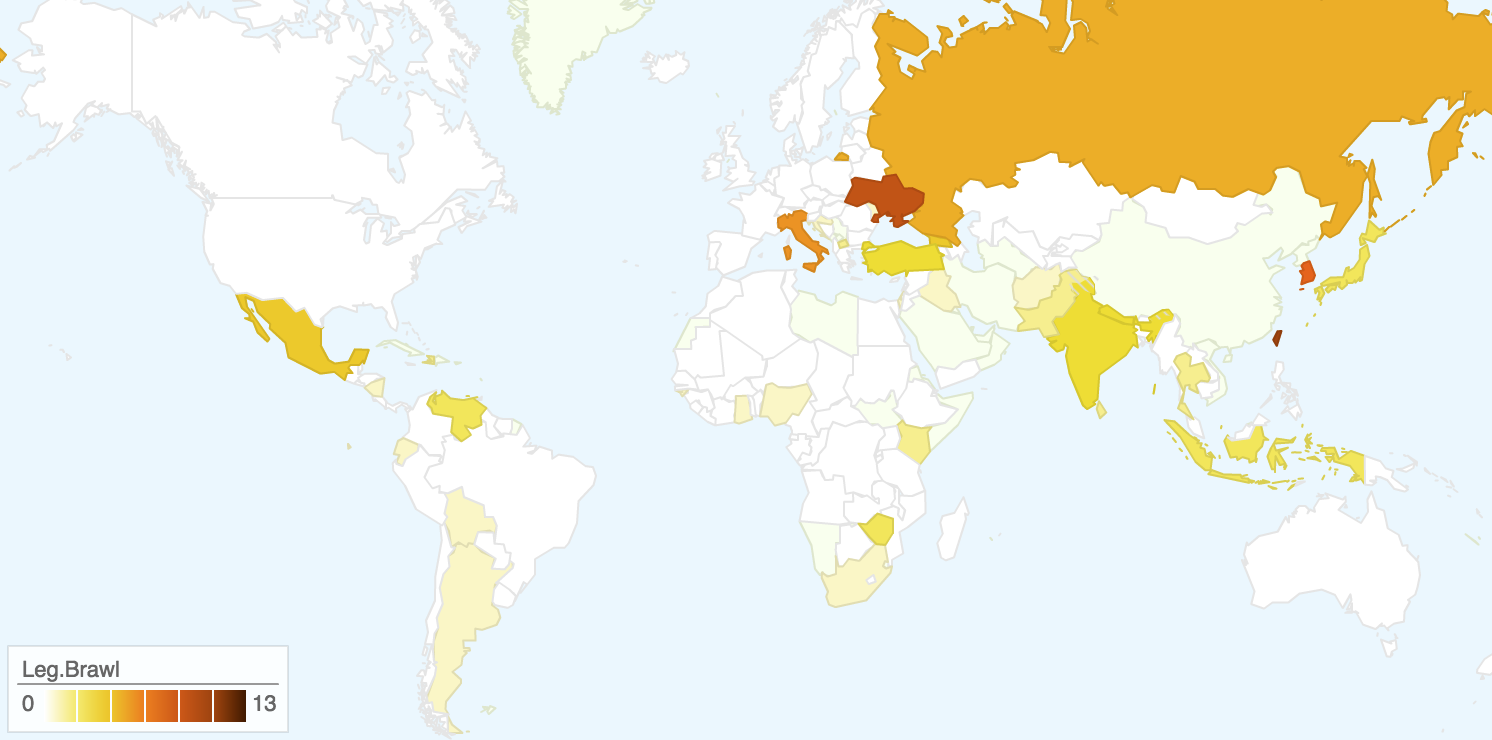
\includegraphics[width = 13cm]{incidence_map.png}
%DIFDELCMD < \end{figure}
%DIFDELCMD < %%%
\DIFdelend \DIFaddbegin \vspace{0.5cm}
\DIFaddend 

\DIFaddbegin \textbf{\DIFadd{FIGURE 1 ABOUT HERE}}

\vspace{0.5cm}

\DIFaddend %%%%%%%%%%%%%% Describing violence in National Legislatures
\DIFdelbegin \section{\DIFdel{Describing Violence in National Legislative Chambers Around the World (1981-2011)}}
%DIFAUXCMD
\addtocounter{section}{-1}%DIFAUXCMD
\DIFdelend \DIFaddbegin \section*{\DIFadd{Describing Violence in National Legislative Chambers Around the World (1981-2012)}}
\DIFaddend 

In order to \DIFdelbegin \DIFdel{further }\DIFdelend systematically explore the causes of legislative violence across the contemporary globe\DIFdelbegin \DIFdel{I primarily used }\DIFdelend \DIFaddbegin \DIFadd{, I used keyword searches of }\DIFaddend the Google News Archive \DIFdelbegin \DIFdel{\mbox{%DIFAUXCMD
\citep{GoogleNews2011}
}%DIFAUXCMD
, which has a global coverage of news sources, }\DIFdelend \DIFaddbegin \DIFadd{LexisNexis, NewsLibrary, NewsBank, general Google Search, and YouTube }\DIFaddend to create a data set of {\emph{physical fights between legislators in national legislative chambers}}. \DIFdelbegin %DIFDELCMD < \endnote{The Google News Archive search was conducted in Spring 2011. A research assistant and I searched using terms that included `national' `parliament', `legislature', `assembly', `brawls', `scuffles', `fights'.} %%%
\DIFdel{This search was }\DIFdelend \DIFaddbegin \DIFadd{See the Online Appendix for details. These searches were }\DIFaddend supplemented by information from colleagues resulting in a data set of \DIFdelbegin \DIFdel{91 }\DIFdelend \DIFaddbegin \DIFadd{131 }\DIFaddend incidents of legislative violence\DIFdelbegin \DIFdel{in 32 countries }\DIFdelend \DIFaddbegin \DIFadd{, 86 of which were in 30 democracies }\DIFaddend between 1981 and \DIFdelbegin \DIFdel{Winter 2011. }\DIFdelend \DIFaddbegin \DIFadd{2012.
}

\DIFaddend We can see in Figure \ref{leg_map} that these events have occurred in many regions around the world. They do not appear to be confined to any one cultural group or region as a simple regional culture explanation would predict. Violence is nonetheless not evenly distributed across countries as we might expect if it was purely the result of legislators with violent personalities. Although I observed \DIFdelbegin \DIFdel{32 countries }\DIFdelend \DIFaddbegin \DIFadd{30 democracies }\DIFaddend having legislative violence, about 60\DIFdelbegin \DIFdel{percent }\DIFdelend \DIFaddbegin \DIFadd{\% }\DIFaddend of these fights occurred in \DIFdelbegin \DIFdel{eight }\DIFdelend \DIFaddbegin \DIFadd{seven }\DIFaddend countries with four or more legislative brawls. These countries include\DIFdelbegin \DIFdel{Ukraine, Mexico}\DIFdelend \DIFaddbegin \DIFadd{: India, Italy}\DIFaddend , South Korea, \DIFdelbegin \DIFdel{and Taiwan}\DIFdelend \DIFaddbegin \DIFadd{Mexico, Taiwan, Turkey, and Ukraine}\DIFaddend .

Before moving on to the regression analysis it is useful to first examine the simple associations between proportional electoral outcomes, democratic age, and violence in this data. Figure \ref{framework_empirical} plots variables measuring these concepts in the entire sample of countries. In the following parametric analysis we will only look at \DIFdelbegin \DIFdel{multi-party elected }\DIFdelend \DIFaddbegin \DIFadd{democratic }\DIFaddend legislatures. Each point represents a country-year. It's notable that virtually every observed incidence of violence took place in legislatures with more disproportionate seat distributions. Similarly, older democracies (approximately 55 years or older) were never observed having legislative brawls in the chamber. See below for details about how disproportionality and democratic age are measured.

While it appears that having disproportionate electoral outcomes \emph{or} a new democracy is not necessary for legislative violence, based on the data, having \emph{both} of them might make violence much more likely. South Korea's national assembly, like the antebellum US Senate, is an example of a `perfect storm'. It is both in a new democracy and has relatively disproportionate electoral outcomes.\footnote{South Korea’s average disproportionality as measured by the Gallagher Index \citep{Gallagher1991} from 2000 until \DIFdelbegin \DIFdel{2011 }\DIFdelend \DIFaddbegin \DIFadd{2012 }\DIFaddend was \DIFdelbegin \DIFdel{12.7. }\DIFdelend \DIFaddbegin \DIFadd{12. }\DIFaddend This places it in the upper 25\DIFdelbegin \DIFdel{percent }\DIFdelend \DIFaddbegin \DIFadd{\% }\DIFaddend of observations with elected legislatures. It also became a democracy within the past 20 years.} South Korea had eight observed incidence of legislative violence in the full sample. Countries that have \emph{either} proportional outcomes \emph{or} old democracies appear to be able to compensate fairly well for an absence of the other characteristic. The United Kingdom has a relatively disproportionate electoral system,\footnote{It had an average Gallagher disproportionality of 16.5 from 2000 to \DIFdelbegin \DIFdel{2011.}\DIFdelend \DIFaddbegin \DIFadd{2012.}\DIFaddend } but no violence in the sample. One reason for this might be that it has a very old democracy where the major parties have had experience in government and so view commitments to allow for the alteration of power to be credible. Conversely, only one incident of violence\footnote{Two members of parliament punched each other in 1998.} was observed in South Africa's new democracy \DIFaddbegin \DIFadd{during the sampling period}\DIFaddend . South Africa's democracy is about the same age as South Korea's and the country has a very violent recent past and present,\footnote{Its rate of murders per 100,000 people is regularly among the highest in the \cite{UNMurder2013} data set.} but it has very proportionate electoral outcomes.\footnote{South Africa’s average disproportionality was \DIFdelbegin \DIFdel{0.29 }\DIFdelend \DIFaddbegin \DIFadd{0.28 }\DIFaddend from 2000 until \DIFdelbegin \DIFdel{2011}\DIFdelend \DIFaddbegin \DIFadd{2012}\DIFaddend , one of the lowest observed in the sample.} South Africa's one scuffle in 1998 is quite an outlier as it is the only violent incident observed in very proportional legislatures in the sample.\DIFaddbegin \footnote{\DIFadd{There was a scuffle in the South African legislature on 12 February 2015, when opposition legislators were being ejected for interrupting the president \mbox{%DIFAUXCMD
\citep{Guardian2015}
}%DIFAUXCMD
. Though South Africa has very proportionate electoral outcomes, the ANC's uninterrupted rule since the end of Apartheid is perhaps beginning to test opposition legislators' belief that the majority can maintain its commitments, especially to alternate power.}}
\DIFaddend 

This brief tour of descriptive statistics adds to the evidence from the previous case study suggesting that violence between legislators does not occur randomly or is confined to one cultural region. Instead violence does appear to be a characteristic of countries with disproportionate electoral outcomes and new democracies.

%DIF < %%%%%%%%%%%%%%% Scatterplot of Disproportionality, AgeDem, and Violence %%%%%%%%%%%%%%%%%%%%%%%%
\DIFdelbegin %DIFDELCMD < \begin{figure}[t]
%DIFDELCMD <     %%%
%DIFDELCMD < \caption{%
{%DIFAUXCMD
\DIFdel{Scatter plots of Disproportionality, Age of Democracy, and Violence in the Full Sample.}}
    %DIFAUXCMD
%DIFDELCMD < \label{framework_empirical}
%DIFDELCMD <     \begin{center}
%DIFDELCMD < %%%
\DIFdelend \DIFaddbegin \vspace{0.5cm}
\DIFaddend 

\DIFdelbegin %DIFDELCMD < \begin{knitrout}
%DIFDELCMD < \definecolor{shadecolor}{rgb}{0.969, 0.969, 0.969}\color{fgcolor}
%DIFDELCMD < 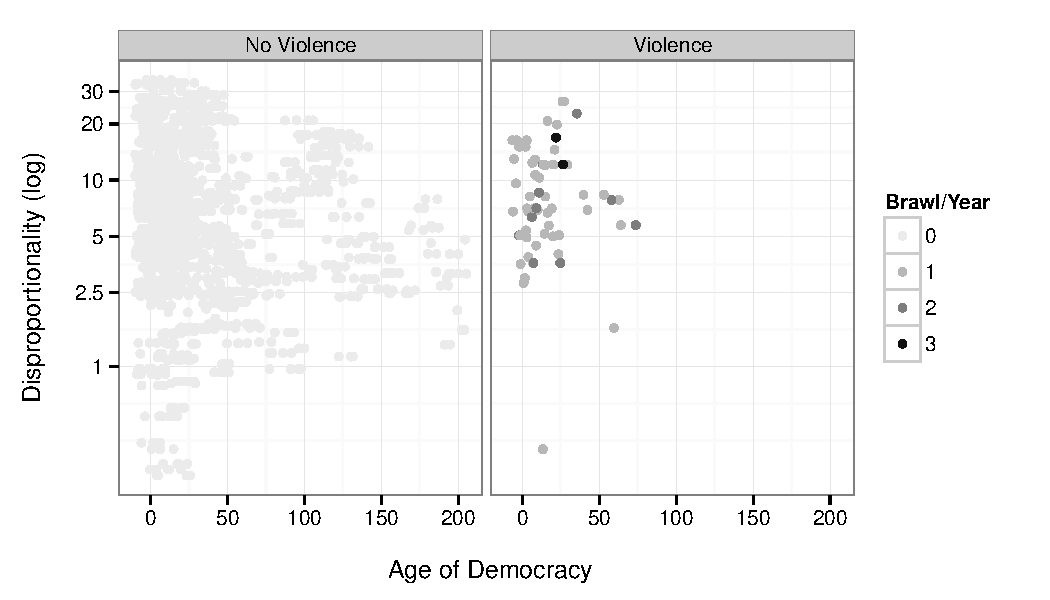
\includegraphics[width=0.8\linewidth]{figure/FrameworkEmpirical-1}
%DIFDELCMD < %%%
\DIFdelend \DIFaddbegin \textbf{\DIFadd{FIGURE 2 ABOUT HERE}}
\DIFaddend 

\DIFdelbegin %DIFDELCMD < \end{knitrout}
%DIFDELCMD <     \end{center}
%DIFDELCMD <     \begin{singlespace}
%DIFDELCMD <         {\scriptsize{Each point represents a country-year. The data is from a sample of 200 countries from 1981 through 2009 due to data availability. The points are jittered horizontally.}}
%DIFDELCMD <     \end{singlespace}
%DIFDELCMD < %%%
\DIFdelend \DIFaddbegin \vspace{0.5cm}
\DIFaddend 

\DIFdelbegin %DIFDELCMD < \end{figure}
%DIFDELCMD < 

%DIFDELCMD < %%%
%DIF < %%%%%%%%%%%%%%% Run Analyses %%%%%%%%%%%%%%%%%%%%%%%%
%DIFDELCMD < 

%DIFDELCMD < %%%
\DIFdelend %%%%%%%%%%%%%%%%%%%%%%%%%%%%%%%%%%%%%%%%%%%%%%%%%%%%%%%%%%%%%%%%%%%%%%%%%%% Empirical Analysis
\DIFdelbegin \section{\DIFdel{Parametric Analysis: Set up}}
%DIFAUXCMD
\addtocounter{section}{-1}%DIFAUXCMD
\DIFdelend \DIFaddbegin \section*{\DIFadd{Parametric Analysis: Set up}}
\DIFaddend 

To more closely and robustly investigate these findings I use incidences of legislative brawls in \DIFdelbegin \DIFdel{multi-party elected }\DIFdelend \DIFaddbegin \DIFadd{democratic }\DIFaddend legislative chambers per country-year\footnote{Country-years with more than one act of violence are given multiple records. See below for how standard errors were adjusted to address statistical issues related to this.} as the dependent variable in a series of regression models \citep{KingRareEvents2001, KingRareEventsPA2001}. All country-years for which data is available over the observation period, regardless of legislative violence, are included in the sample. \DIFdelbegin \DIFdel{Data on whether or not a legislature had multiple elected parties is from the Database of Political Institutions (DPI) \mbox{%DIFAUXCMD
\citep[updated to 2010]{DPI2001}
}%DIFAUXCMD
}%DIFDELCMD < {%%%
\emph{\DIFdel{Legislative Indices of Electoral Competitiveness}}%DIFAUXCMD
%DIFDELCMD < } %%%
\DIFdel{variable. Due to a lack of data on some of the co-variates discussed below, I also constricted the sample to years before 2010. This reduced the number of incidence from 99 to 77. Full replication data and code used for all of the analyses can be found in this paper's source code files}\DIFdelend \DIFaddbegin \DIFadd{Countries-years were deemed to be democratic if their Polity IV score \mbox{%DIFAUXCMD
\citep{Marshall2009}
}%DIFAUXCMD
was greater than five, the point above which that data set's creators classify a country as democratic}\DIFaddend .

%%%%%%%%%%%%%%%%%%%%%%%%%%%%%%%%%%%%%%%%%%%% Empirical Model
\DIFdelbegin \subsection{\DIFdel{Parametric Models}}
%DIFAUXCMD
\addtocounter{subsection}{-1}%DIFAUXCMD
\DIFdelend \DIFaddbegin \subsection*{\DIFadd{Parametric Models}}
\DIFaddend 

Legislative brawls are rare. Most of the time the overwhelming majority of legislatures do not have physical fights. The rarity of legislative brawls creates some empirical problems. Standard logistic regression techniques can ``sharply underestimate the probability of rare events" \cite[137]{KingRareEventsPA2001}. Estimated regression coefficients from logistic regression analysis with many fewer observed events than non-events will be too small. Furthermore, standard methods for computing event probabilities with logistic regression produce results biased in the same direction as the coefficient estimates. To overcome this problem \cite{KingRareEvents2001,KingRareEventsPA2001} propose a bias-corrected logistic model for rare events data--rare events logistic regression. I use this method below.

%%%%%%%%%%%%%%%%%%%%%%%%%%%%%%%%%%%%%%%%%%%% Independent variables
\DIFdelbegin \subsection{\DIFdel{Right-hand Variables}}
%DIFAUXCMD
\addtocounter{subsection}{-1}%DIFAUXCMD
\DIFdelend \DIFaddbegin \subsection*{\DIFadd{Right-hand Variables}}
\DIFaddend 

I included a number of political and societal variables in the regression models to test if the associations we saw earlier are actually spurious. Variable descriptions and sources are summarized in a table that can be found in the Supplementary Material. In the interest of transparency, the table includes all of the variables that I have included in all versions of the models, even those not shown because they did not generate substantively or statistically meaningful results. A matrix illustrating the variables' correlations can also be found in the Supplementary Material. This figure includes the variables' observed minimum and maximum values for reference.

I measure the {\emph{age of a democratic regime}} as the number of years a country's Polity IV score \citep{Marshall2009} is greater than five\DIFdelbegin \DIFdel{, the point above which that data set's creators classify a country as democratic. I use two variables to examine the relationship between the proportionality of electoral outcomes and violence. One is purely institutional: a simple dummy of whether or not a country's legislature is elected by some form of }%DIFDELCMD < {%%%
\emph{\DIFdel{proportional electoral system}}%DIFAUXCMD
%DIFDELCMD < }%%%
\DIFdel{. The variable is from the DPI database}\DIFdelend . \DIFaddbegin \DIFadd{Because this variable is highly right-skewed, I transformed it using the natural logarithm. }\DIFaddend As noted earlier, simply looking at the electoral mechanics confuses mechanisms with outcomes. So, \DIFdelbegin \DIFdel{more importantly, }\DIFdelend I use the standard Least Squares or Gallagher Index \citep{Gallagher1991} to measure realized {\emph{electoral disproportionality}}. The available data is in terms of overall national disproportionality. To gain maximum coverage, I compiled the data from both \cite{Gallagher2012} and \cite{Carey2011}. Full details can be found at: \DIFdelbegin %DIFDELCMD < \url{http://christophergandrud.github.com/Disproportionality_Data/}%%%
\DIFdelend \DIFaddbegin [\DIFadd{WITHHELD FOR BLIND REVIEW}]
%DIF >  \url{http://christophergandrud.github.com/Disproportionality_Data/}
\DIFaddend .
A country's disproportionality score is treated as constant from the year of an election until the year before the following election. Higher values on the Gallagher Index indicate more disproportionate, i.e. less fair electoral outcomes.

As we saw in Figure \ref{framework_empirical} there appears to be a very strong negative correlation between very low levels of disproportionality and legislative violence. Only one instance of violence was observed in countries with a disproportionality score of less than about 2.5.\footnote{Though the observed range of disproportionality scores goes from almost 0 to 30, countries with scores less than 2.5 are not outliers. About \DIFdelbegin \DIFdel{42 percent }\DIFdelend \DIFaddbegin \DIFadd{16\% }\DIFaddend of county-years in the \DIFaddbegin \DIFadd{full }\DIFaddend sample had scores of 2.5 or smaller.} This can be explained by fairness equilibria and is partially corroborated by Marien's \citeyearpar{Marien2011} finding regarding very low disproportionality measured with the Gallagher Index and political trust discussed above. To capture a possible disproportionality threshold effect--where low disproportionality is associated with stronger feelings of fairness--I created a low disproportionality dummy variable. County-years with disproportionality greater than or equal to the observed median \DIFdelbegin \DIFdel{(6}\DIFdelend \DIFaddbegin \DIFadd{in the full sample (6.34}\DIFaddend )\footnote{The observed range is 0.26 to 34.52.} are coded as having higher disproportionality and those with scores lower than \DIFdelbegin \DIFdel{6 }\DIFdelend \DIFaddbegin \DIFadd{6.34 }\DIFaddend are coded as having lower disproportionality.\footnote{\DIFdelbegin \DIFdel{Models }\DIFdelend \DIFaddbegin \DIFadd{Medians of other sample subsets, such as all country-years with democratic legislatures, }\DIFaddend were \DIFaddbegin \DIFadd{also examined. The results were substantively similar. Additional models were }\DIFaddend estimated with the continuous disproportionality measure. The parameter estimates were not statistically significant and are not shown.}

I also investigated the possibility that a number of political, institutional, and cultural variables may actually be associated with legislative violence and that the key variables from my argument actually have spurious associations. To get a sense of how the size of the governing majority is associated with legislative violence I include the government {\emph{majority}} variable (from the DPI). It simply measures the seats held by governing parties as a proportion of all seats. I transformed the variable from a proportion to a\DIFdelbegin \DIFdel{percentage }\DIFdelend \DIFaddbegin \DIFadd{\%age }\DIFaddend to ease interpretation. Legislators may be less likely to attack one another if they know that they could be arrested for assault. To examine this possibility I include Fish and Koening's \citeyearpar{Fish2009} dichotomous \emph{legislator immunity} variable. It equals one if national legislators are immune from arrest and/or prosecution and zero otherwise. Unfortunately, their data only captures legislative immunity in 2007. I extrapolated the 2007 value of the variable to the other observation years.\footnote{I also considered using the legislator immunity variable from the Comparative Constitutions Project \citep{ElkinsCCP2010}. However, the coding of the immunity variable is vaguer than Fish and Koening's and only deals with constitutionally mandated immunity.} We should therefore approach results from this variable with caution since it might not be a valid indicator for all country-years.

To \DIFdelbegin \DIFdel{examine the relationships between societal-level values and legislative violence I rely primarily on data from the World Values Survey \mbox{%DIFAUXCMD
\citeyearpar{WVS2009}
}%DIFAUXCMD
. Over the course of his research, Ingelhart has found that his composite }%DIFDELCMD < {%%%
\emph{\DIFdel{self-expression}}%DIFAUXCMD
%DIFDELCMD < } %%%
\DIFdel{indicator is the best way to capture cultural and normative differences between democracies and non-democracies. Societies have high self-expression scores if they emphasize ``liberty and participation, public self-expression, tolerance of diversity, interpersonal trust, and life satisfaction" \mbox{%DIFAUXCMD
\citep[64]{Inglehart2003}
}%DIFAUXCMD
. So I include the self-expression variable from the World Values Survey.}\footnote{\DIFdel{In earlier versions of the models I also included components of this variable. However, they were either never statistically significant or produced unintelligible and unstable results.}} %DIFAUXCMD
\addtocounter{footnote}{-1}%DIFAUXCMD
\DIFdel{Following \mbox{%DIFAUXCMD
\cite{Inglehart2003}
}%DIFAUXCMD
I average the variables across individual participants within countries and survey waves. I only use the third through fifth survey waves}\footnote{\DIFdel{The surveys were taken in the following years: }%DIFDELCMD < \\ %%%
\DIFdel{Wave 3: 1994--1998 }%DIFDELCMD < \\ %%%
\DIFdel{Wave 4: 1999--2004 }%DIFDELCMD < \\ %%%
\DIFdel{Wave 5: 2005--2007}} %DIFAUXCMD
\addtocounter{footnote}{-1}%DIFAUXCMD
\DIFdel{as the first two waves have very poor coverage. I used wave 3 for all years before 1998, wave 4 for all years between 1999 and 2004 and wave 5 onward.
}%DIFDELCMD < 

%DIFDELCMD < %%%
\DIFdel{Gender is closely correlated with violence in society generally. Though there are many possible reasons for this that are beyond the scope of this paper, women tend to commit many fewer acts of violence than men \mbox{%DIFAUXCMD
\citep[see][]{Schwartz2009}
}%DIFAUXCMD
. Previous research has found that women's participation in parliament has an impact on government decisions to go to war \mbox{%DIFAUXCMD
\citep{Melander2005}
}%DIFAUXCMD
. Perhaps if a larger proportion of legislators are women there will be less violence in the parliamentary chamber. To examine this possibility, I gathered data on the }\emph{\DIFdel{percentage of women in parliament}} %DIFAUXCMD
\DIFdel{per country-year from two sources. Data from 1997 and after was from the Inter-Parliamentary Union \mbox{%DIFAUXCMD
\citeyearpar{IPU2013}
}%DIFAUXCMD
. Data from before 1997 was from \mbox{%DIFAUXCMD
\cite{Schwartz2009}
}%DIFAUXCMD
.
}%DIFDELCMD < 

%DIFDELCMD < %%%
\DIFdel{I included a countries' }\emph{\DIFdel{murder rate}}%DIFAUXCMD
\DIFdel{, i.e. murders per 100,000 people, to measure a possible association between societal-level and legislative violence. The data was from \mbox{%DIFAUXCMD
\cite{UNMurder2013}
}%DIFAUXCMD
, which aggregated annual murder rates from a variety of national and international sources. The data is available from 1995 through 2011.}\footnote{\DIFdel{Beyond truncating the sample somewhat, this data set unfortunately does not record Taiwan's murder rate separately from China's.}}
%DIFAUXCMD
\addtocounter{footnote}{-1}%DIFAUXCMD
%DIFDELCMD < 

%DIFDELCMD < %%%
\DIFdel{To }\DIFdelend assess any effect of coalition compared to single-party governments I included the DPI {\emph{government fractionalization}} variable. It is the probability that two randomly picked deputies in the government are from different parties. I used the fractionalization variable to create an indicator of {\emph{single-party}} government. It is simply a dummy equaling one if fractionalization was zero, i.e. all governing legislators were from the same party. In general single party governments probably are better able to pass policies very close to their ideal preferences. This could heighten losers' losses and make them less likely to want to conform to non-violent legislative rules. However, all single party governments are not created equal. Some parties may act as umbrella parties that incorporate many different factions. Others are narrowly focused on a particular constituency.

\DIFdelbegin \DIFdel{I also included standard measures of the }\emph{\DIFdel{effective number of parliamentary parties}} %DIFAUXCMD
\DIFdel{by votes and by seats \mbox{%DIFAUXCMD
\citep[see][]{Laakso1979, Taagepera1989}
}%DIFAUXCMD
.The data was taken from \mbox{%DIFAUXCMD
\cite{Carey2011}
}%DIFAUXCMD
before 2004 and from \mbox{%DIFAUXCMD
\cite{Gallagher2012}
}%DIFAUXCMD
afterwards. Both of these measures indicate how fragmented a parliamentary party system is. Higher scores }\DIFdelend \DIFaddbegin \DIFadd{Perhaps legislators are more violent if they become frustrated with their ability to effect policy change. Control over legislative resources typically closely corresponds to an ability to shape outcomes. However, veto players outside the legislature may severely restrict what bills pass the legislature are actually enacted. To examine this possibility, I included Henisz's \mbox{%DIFAUXCMD
\citeyearpar{Henisz2004}
}%DIFAUXCMD
measure of political constraints.}\footnote{\DIFadd{The version of the variable included is POLCONIII. Results are similar for the other version--POLCONV--which includes two additional veto points: the judiciary and sub-federal units.}} \DIFadd{This variable captures the feasibility of policy change. It ranges between 0 and 1. Higher values }\DIFaddend indicate that there are more \DIFdelbegin \DIFdel{parties that win either votes or seats. Neither measure produced statistically significant results, so only the results for the effective number of parties by seats are shown below.
}\DIFdelend \DIFaddbegin \DIFadd{veto players with disparate preferences. The variable has been updated through 2011.
}\DIFaddend 

To examine \DIFdelbegin \DIFdel{whether or not national legislative losers may be dissuaded from legislative violence because there is a possibility of gaining power at a provincial-level, I include the }\emph{\DIFdel{federalism}} %DIFAUXCMD
\DIFdel{dummy variable from \mbox{%DIFAUXCMD
\cite{Carey2011}
}%DIFAUXCMD
.
}\DIFdelend \DIFaddbegin \DIFadd{the possibility that armed conflict may be associated with legislative violence }\DIFaddend I \DIFdelbegin \DIFdel{updated this from }\DIFdelend \DIFaddbegin \DIFadd{created a binary internal armed conflict variable using the UCDP/PRIO Armed Conflict Dataset \mbox{%DIFAUXCMD
\citep{Themner2014}
}%DIFAUXCMD
. The variable is one if there is an internal armed conflict (either involving or not involving external states) and zero otherwise.
}


\DIFadd{To examine the relationships between societal-level values and legislative violence I rely primarily on data from the World Values Survey \mbox{%DIFAUXCMD
\citeyearpar{WVS2009}
}%DIFAUXCMD
. Over the course of his research, Ingelhart has found that his composite }{\emph{\DIFadd{self-expression}}} \DIFadd{indicator is the best way to capture cultural and normative differences between democracies and non-democracies. Societies have high self-expression scores if they emphasize ``liberty and participation, public self-expression, tolerance of diversity, interpersonal trust, and life satisfaction" \mbox{%DIFAUXCMD
\citep[64]{Inglehart2003}
}%DIFAUXCMD
. So I include the self-expression variable from the World Values Survey.}\footnote{\DIFadd{In earlier versions of the models I also included components of this variable. However, they were either never statistically significant or produced unintelligible and unstable results.}} \DIFadd{Following \mbox{%DIFAUXCMD
\cite{Inglehart2003}
}%DIFAUXCMD
I average the variables across individual participants within countries and survey waves. I only use the third through fifth survey waves}\footnote{\DIFadd{The surveys were taken in the following years: }\\ \DIFadd{Wave 3: 1994--1998 }\\ \DIFadd{Wave 4: 1999--2004 }\\ \DIFadd{Wave 5: 2005--2007}} \DIFadd{as the first two waves have very poor coverage. I used wave 3 for all years before 1998, wave 4 for all years between 1999 and }\DIFaddend 2004 \DIFdelbegin \DIFdel{until the end of the observation period. In early models I also controlled for the government system type, i. e. if it had a presidential, parliamentary, or mixed assembly-elected presidential. This was from the DPI.}%DIFDELCMD < 

%DIFDELCMD < %%%
\DIFdel{I include a number of other societal-level variables to help further defend against omitted variable bias. Conflict }\DIFdelend \DIFaddbegin \DIFadd{and wave 5 onward.
}

\DIFadd{In addition, competition }\DIFaddend in more ethnically \DIFdelbegin \DIFdel{or economically }\DIFdelend divided societies may be generally more intense. These conflicts may spill over into legislatures where they precipitate violence between members. I include Alesina et al.'s \citeyearpar{Alesina2003} {\emph{ethnic fractionalization}} data to account for the fact that a legislature's composition in terms of its fractionalization is not only a function of political institutions, but also social divisions \citep{Neto1997, Mozaffar2003}. The variable measures the probability that two randomly selected members of society will be from different ethnic groups. Higher values indicate more \DIFdelbegin \DIFdel{societal fractionalization.
To capture similar possible effects from economic divisions, I include }%DIFDELCMD < {%%%
\emph{\DIFdel{Gini coefficients of economic inequality}}%DIFAUXCMD
%DIFDELCMD < } %%%
\DIFdel{from \mbox{%DIFAUXCMD
\cite{UNU2008}
}%DIFAUXCMD
. }\footnote{\DIFdel{Note, for country-years with missing data I assumed that the Gini Coefficient remained constant from the last year there is data for the country, unless the span was ten years or more. If this was the case they were treated as missing.}} %DIFAUXCMD
\addtocounter{footnote}{-1}%DIFAUXCMD
\DIFdel{Finally, as is common in cross-country analyses, I also include }%DIFDELCMD < {%%%
\emph{\DIFdel{gross domestic product per capita}}%DIFAUXCMD
%DIFDELCMD < }%%%
\DIFdel{. This data is from the World Bank's International Development Indicators \mbox{%DIFAUXCMD
\citeyearpar{WorldBank2011}
}%DIFAUXCMD
and is in thousands of United States dollars}\DIFdelend \DIFaddbegin \DIFadd{fractionalization}\DIFaddend .

\DIFaddbegin \DIFadd{Please see the Online Appendix for discussions of and results for a number of other variables that were tested to examine the possibility of omitted variable bias. These variables include: the\%age of women in parliament, murder rates, government fractionalization, the effective number of parties in the legislature, federalism, the Gini coefficient, and GDP per capita.
}

\DIFaddend %%%%%%%%%%%%%%%%%%%%%%%%%%%%%%%%%%%%%%%%%%%% Analyses


\DIFdelbegin \section{\DIFdel{Regression Results}}
%DIFAUXCMD
\addtocounter{section}{-1}%DIFAUXCMD
\DIFdelend \DIFaddbegin \section*{\DIFadd{Regression Results}}
\DIFaddend 

I used the {\tt{relogit}} model from the {\tt{R}} package Zelig \citep{IMAIKingZelig2008} to estimate regression models. Furthermore, to get a better understanding of the magnitude of the estimated relationships between the right-hand variables and violence, I also used Zelig to predict incident probabilities with \DIFdelbegin \DIFdel{1000 }\DIFdelend \DIFaddbegin \DIFadd{1,000 }\DIFaddend simulations per fitted value \DIFdelbegin \DIFdel{\mbox{%DIFAUXCMD
\citep[see][]{King2002}
}%DIFAUXCMD
. Predicted }\DIFdelend \DIFaddbegin \DIFadd{\mbox{%DIFAUXCMD
\citep[]{King2002}
}%DIFAUXCMD
. Expected }\DIFaddend probabilities for various fitted values of the key findings of interest with robust results are shown in Figure \ref{pred_prob}. These give us a substantively meaningful sense of estimated effects' magnitudes. Note: because the variables are in country-year records, all of the results should be interpreted in terms of the predicted effect of a variable on the probability of legislative violence in a given country in a year.

I observed relatively few incidences of violence in the 1980s.\footnote{There were only 8 observed incidence before \DIFdelbegin \DIFdel{1990.}\DIFdelend \DIFaddbegin \DIFadd{1990 in the full sample.}\DIFaddend } This may be because news articles from before the 1990s have not been made available on the internet with the same frequency as those written from the 1990s. To examine any estimation biases this sampling bias might create I ran the regressions on a further constricted sample of \DIFdelbegin \DIFdel{multi-party elected }\DIFdelend \DIFaddbegin \DIFadd{democratic }\DIFaddend legislatures from 1990. The results were broadly similar across the two samples. Regression coefficient point estimates and robust standard errors for the sample that is truncated from 1990 can be found in Table \ref{outputTable.1990}. Results from the full observation period can be found in the \DIFdelbegin \DIFdel{Supplementary Material. }\DIFdelend \DIFaddbegin \DIFadd{Online Appendix. In addition, the Online Appendix contain a further examination of why more incidents are observed in more recent time periods.
}\DIFaddend 

Individual observations are clearly correlated within countries and years, especially when there were multiple acts of violence in a country in a year. To address this issue I used robust standard errors \citep{Golder2006, Mainwaring2007}. Standard errors were adjusted using \cite{Lumley1999} weighted empirical adaptive variance estimators (WEAVE) where the true dependence structure does not need to be specified prior to running the analysis.

%DIF < %%%%%%% Elected Legislatures Results Table from 1990
\DIFdelbegin %DIFDELCMD < \begin{table}
%DIFDELCMD < %%%
%DIFDELCMD < \caption{%
{%DIFAUXCMD
\DIFdel{Legislative Violence Regression Results (Multi-Party Elected Legislature from 1990-2009)}}
%DIFAUXCMD
%DIFDELCMD < \label{outputTable.1990}
%DIFDELCMD < \begin{center}
%DIFDELCMD < \scalebox{0.9}{
%DIFDELCMD < 

%DIFDELCMD < \begin{tabular}{l c c c c c c c c }
%DIFDELCMD < \hline
%DIFDELCMD <                         & A1 & A2 & A3 & A4 & A5 & A6 & A7 & A8 \\
%DIFDELCMD < \hline
%DIFDELCMD < (Intercept)             & $-2.70^{***}$ & $-0.98$       & $-4.32$      & $-1.34$     & $-2.19^{**}$ & $-1.80^{*}$  & $-1.85^{*}$  & $-2.20^{*}$  \\
%DIFDELCMD <                         & $(0.21)$      & $(0.80)$      & $(4.47)$     & $(0.71)$    & $(0.85)$     & $(0.84)$     & $(0.79)$     & $(1.11)$     \\
%DIFDELCMD < Low Disproportionality  & $-1.12^{**}$  & $-1.33^{***}$ & $-1.81^{**}$ & $-0.91^{*}$ & $-1.27^{*}$  & $-1.53^{**}$ & $-1.16^{**}$ & $-1.05^{**}$ \\
%DIFDELCMD <                         & $(0.36)$      & $(0.37)$      & $(0.63)$     & $(0.41)$    & $(0.53)$     & $(0.57)$     & $(0.39)$     & $(0.40)$     \\
%DIFDELCMD < Dem. Age                & $-0.02^{**}$  & $-0.03^{**}$  & $-0.03$      & $-0.02^{*}$ & $-0.03^{*}$  & $-0.03^{*}$  & $-0.03^{**}$ & $-0.04^{*}$  \\
%DIFDELCMD <                         & $(0.01)$      & $(0.01)$      & $(0.01)$     & $(0.01)$    & $(0.01)$     & $(0.01)$     & $(0.01)$     & $(0.02)$     \\
%DIFDELCMD < Majority Size           &               & $-0.03^{**}$  & $-0.03$      & $-0.02^{*}$ & $-0.00$      & $-0.02$      & $-0.03^{*}$  & $-0.03^{*}$  \\
%DIFDELCMD <                         &               & $(0.01)$      & $(0.02)$     & $(0.01)$    & $(0.01)$     & $(0.01)$     & $(0.01)$     & $(0.01)$     \\
%DIFDELCMD < Leg. Immunity           &               & $-0.20$       &              &             &              &              &              &              \\
%DIFDELCMD <                         &               & $(0.36)$      &              &             &              &              &              &              \\
%DIFDELCMD < PR Electoral System     &               & $0.74$        &              &             &              &              &              &              \\
%DIFDELCMD <                         &               & $(0.53)$      &              &             &              &              &              &              \\
%DIFDELCMD < Single Party Gov.       &               & $-0.64$       &              &             &              &              &              &              \\
%DIFDELCMD <                         &               & $(0.35)$      &              &             &              &              &              &              \\
%DIFDELCMD < Self Expression         &               &               & $2.51$       &             &              &              &              &              \\
%DIFDELCMD <                         &               &               & $(3.59)$     &             &              &              &              &              \\
%DIFDELCMD < Ethnic Frac.            &               &               & $0.89$       &             &              &              &              &              \\
%DIFDELCMD <                         &               &               & $(1.23)$     &             &              &              &              &              \\
%DIFDELCMD < Perc. Women in Parl.    &               &               &              & $-0.02$     &              &              &              &              \\
%DIFDELCMD <                         &               &               &              & $(0.02)$    &              &              &              &              \\
%DIFDELCMD < Murder Rate             &               &               &              &             & $0.01$       &              &              &              \\
%DIFDELCMD <                         &               &               &              &             & $(0.02)$     &              &              &              \\
%DIFDELCMD < Federal                 &               &               &              &             &              & $0.74$       & $0.64$       &              \\
%DIFDELCMD <                         &               &               &              &             &              & $(0.60)$     & $(0.46)$     &              \\
%DIFDELCMD < Gov. Frac.              &               &               &              &             &              & $0.79$       &              &              \\
%DIFDELCMD <                         &               &               &              &             &              & $(0.82)$     &              &              \\
%DIFDELCMD < No. of Parties by Seats &               &               &              &             &              &              & $0.13$       &              \\
%DIFDELCMD <                         &               &               &              &             &              &              & $(0.08)$     &              \\
%DIFDELCMD < GINI                    &               &               &              &             &              &              &              & $0.03$       \\
%DIFDELCMD <                         &               &               &              &             &              &              &              & $(0.02)$     \\
%DIFDELCMD < GDP per Capita          &               &               &              &             &              &              &              & $0.03$       \\
%DIFDELCMD <                         &               &               &              &             &              &              &              & $(0.03)$     \\
%DIFDELCMD < \hline
%DIFDELCMD < AIC                     & 370.24        & 356.99        & 178.59       & 302.28      & 191.36       & 176.05       & 299.34       & 288.98       \\
%DIFDELCMD < BIC                     & 386.58        & 395.02        & 205.25       & 328.78      & 215.19       & 204.71       & 331.04       & 319.95       \\
%DIFDELCMD < Log Likelihood          & -182.12       & -171.49       & -83.30       & -146.14     & -90.68       & -82.02       & -143.67      & -138.49      \\
%DIFDELCMD < Deviance                & 364.24        & 342.99        & 166.59       & 292.28      & 181.36       & 164.05       & 287.34       & 276.98       \\
%DIFDELCMD < Num. obs.               & 1714          & 1691          & 628          & 1691        & 1492         & 931          & 1509         & 1458         \\
%DIFDELCMD < \hline
%DIFDELCMD < \multicolumn{9}{l}{\scriptsize{$^{***}p<0.001$, $^{**}p<0.01$, $^*p<0.05$}}
%DIFDELCMD < \end{tabular}
%DIFDELCMD < 

%DIFDELCMD < }
%DIFDELCMD < \end{center}
%DIFDELCMD < {\scriptsize{
%DIFDELCMD <     Standard errors are in parentheses. All models use robust (WEAVE) standard errors. \\
%DIFDELCMD < }}
%DIFDELCMD < \end{table}
%DIFDELCMD < %%%
\DIFdelend \DIFaddbegin \DIFadd{Finally, I subsetted the sample to include only democracies defined as country-years with a Polity IV greater than 5. Results from models with all countries that had elected multi-party legislatures, regardless of their Polity IV score are substantively similar.
}\DIFaddend 

I avoid focusing on models that include highly correlated variables \DIFdelbegin \DIFdel{\mbox{%DIFAUXCMD
\citep[see][]{Achen2002, Schrodt2006}
}%DIFAUXCMD
}\DIFdelend \DIFaddbegin \DIFadd{\mbox{%DIFAUXCMD
\citep[]{Achen2002, Schrodt2006}
}%DIFAUXCMD
}\DIFaddend . In these models (not shown), as the statistical literature predicts, the coefficient estimates and standard errors change dramatically for many of the variables. \DIFdelbegin \DIFdel{There may be interactions between many of the variables included in the models. I attempted to capture interactions in the analysis, but it was empirically difficult. Given the small number of observed incidences of legislative violence there could simply not be enough information in the data to draw meaningful conclusions about these types of relationship \mbox{%DIFAUXCMD
\citep[see][]{Brambor2006}
}%DIFAUXCMD
. I }\DIFdelend \DIFaddbegin \DIFadd{I }\DIFaddend also ignore results from models with the government system type variable. It had very large, highly unstable, and largely nonsensical coefficient estimates, suggesting that the model does not contain enough information to test \citep{Babyak2004} whether or not \DIFaddbegin \DIFadd{crude }\DIFaddend political system type has an effect on violence. \DIFaddbegin \DIFadd{The instability in the coefficient estimates likely has more to do with a lack of variation on this covariates rather than the violence dependent variable. Political system rarely changes in the sample.
}\DIFaddend 

%DIF < %%%%%%%%%%%%%%% Predicted Probability Graphs %%%%%%%%%%%%%%%%%%%%%%%%
\DIFdelbegin %DIFDELCMD < \begin{figure}[t]
%DIFDELCMD <     %%%
%DIFDELCMD < \caption{%
{%DIFAUXCMD
\DIFdel{Predicted Probability of Legislative Violence in Multi-Party Elected Legislatures}}
    %DIFAUXCMD
%DIFDELCMD < \label{pred_prob}
%DIFDELCMD <     \begin{center}
%DIFDELCMD < %%%
\DIFdelend \DIFaddbegin \vspace{0.5cm}
\DIFaddend 

%DIF < \includegraphics[width = \textwidth]{leg_violence_paper-PredProb}
\DIFaddbegin \textbf{\DIFadd{TABLE I ABOUT HERE}}
\DIFaddend 

\DIFdelbegin %DIFDELCMD < \begin{knitrout}
%DIFDELCMD < \definecolor{shadecolor}{rgb}{0.969, 0.969, 0.969}\color{fgcolor}
%DIFDELCMD < 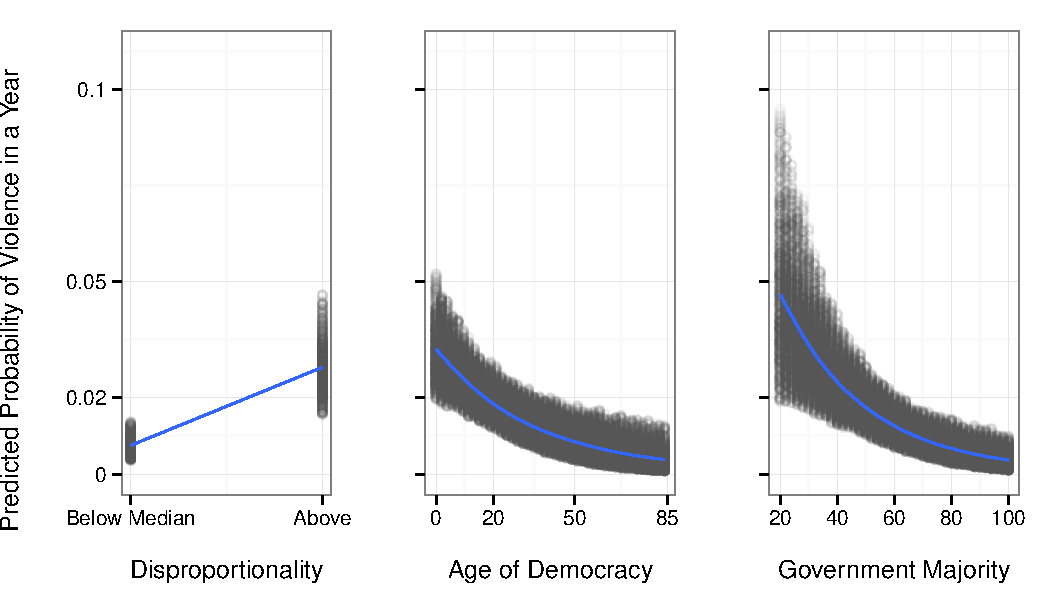
\includegraphics[width=0.8\linewidth]{figure/predProb}
%DIFDELCMD < %%%
\DIFdelend \DIFaddbegin \vspace{0.5cm}
\DIFaddend 


\DIFdelbegin %DIFDELCMD < \end{knitrout}
%DIFDELCMD <     \end{center}
%DIFDELCMD <     \begin{singlespace}
%DIFDELCMD <       {\scriptsize{The graphs show the middle 95\% of 1000 simulations at each fitted value of the variables. The simulations use Model A2, Table \ref{outputTable.1990}. For each set of simulations all other variables were fitted at their means.}}
%DIFDELCMD <     \end{singlespace}
%DIFDELCMD < \end{figure}
%DIFDELCMD < %%%
\DIFdelend \DIFaddbegin \vspace{0.5cm}
\DIFaddend 

\DIFaddbegin \textbf{\DIFadd{FIGURE 3 ABOUT HERE}}

\vspace{0.5cm}


\DIFaddend \paragraph{Disproportionality}

Across \DIFaddbegin \DIFadd{virtually }\DIFaddend all of the models the estimates for the dummy {\emph{low disproportionality}} variable indicate that proportional electoral outcomes are associated with less legislative violence. This finding is robust at least at the 5\% significance level in \DIFdelbegin \DIFdel{all }\DIFdelend \DIFaddbegin \DIFadd{most }\DIFaddend model specifications.\DIFaddbegin \footnote{\DIFadd{The only model in Table \ref{outputTable.1990} where it just drops below the 10\% significance level is Model 6. This model includes the self expression variable which, due to missingness, causes the sample size to be cut almost in half. In the full 1990-2012 sample the coefficient estimate was significant at the 10\% level with self-expression included. Please see the Online Appendix.}} \DIFaddend The finding corroborates what we saw in the Sumner caning case study and Figure \ref{framework_empirical}. Violence is rare in countries with Gallagher scores below the \DIFdelbegin \DIFdel{median--6--and }\DIFdelend \DIFaddbegin \DIFadd{median--6.34--and }\DIFaddend there is something of a cut-off point--around 2.5--below which these highly proportional countries were almost never observed to have had violence. More interesting than simple statistical significance or coefficient point estimates is the magnitude of and uncertainty surrounding the disproportionality/violence relationship. To get a sense of the magnitude of this estimated relationship and the uncertainty around it I plotted the predicted probabilities of having a legislative brawl in the left-most plot of Figure \ref{pred_prob} using estimates from Model \DIFdelbegin \DIFdel{A2. }\DIFdelend \DIFaddbegin \DIFadd{4. }\DIFaddend We can see that the \DIFdelbegin \DIFdel{central tendency of the predicted }\DIFdelend \DIFaddbegin \DIFadd{median of the expected }\DIFaddend probabilities of a country having violence when disproportionality is greater than or equal to \DIFdelbegin \DIFdel{6 is over two percent }\DIFdelend \DIFaddbegin \DIFadd{6.34 is well over three\% }\DIFaddend in a given year. All other variables are fitted at their means. Countries with disproportionality less than \DIFdelbegin \DIFdel{6 }\DIFdelend \DIFaddbegin \DIFadd{6.34 }\DIFaddend had a very low predicted probability of violence in a year.

\paragraph{Age of \DIFdelbegin \DIFdel{Democracy}\DIFdelend \DIFaddbegin \DIFadd{democracy}\DIFaddend }

Also, corroborating the evidence we saw before, the analyses indicate that older democracies tend to have less legislative violence. This result is significant at least at the \DIFdelbegin \DIFdel{10 percent }\DIFdelend \DIFaddbegin \DIFadd{5\% }\DIFaddend level in all of the models. Looking at the middle panel of Figure \ref{pred_prob} we can see that violence is more likely in younger democracies. Very young democracies are predicted to have about a three to four\DIFdelbegin \DIFdel{percent }\DIFdelend \DIFaddbegin \DIFadd{\% }\DIFaddend probability of experiencing legislative violence in a given year. The probability of violence decreases steadily as a democracy ages. The predicted probability of violence becomes largely indistinguishable from zero--i.e. no probability of violence--sometime shortly after a democracy turns 50 years old.

\paragraph{Governing \DIFdelbegin \DIFdel{Majorities}\DIFdelend \DIFaddbegin \DIFadd{majorities}\DIFaddend }

I also found a negative relationship between the size of governments' legislative majorities and violence. We can see in the right-most panel of Figure \ref{pred_prob} that the predicted probability of violence in countries with minority governments is relatively high at about 5\DIFdelbegin \DIFdel{percent }\DIFdelend \DIFaddbegin \DIFadd{\% }\DIFaddend in a year. This is somewhat higher than predicted for countries with high disproportionality or new democracies, though the variance is much larger. This finding fits well within this \DIFdelbegin \DIFdel{paper}\DIFdelend \DIFaddbegin \DIFadd{article}\DIFaddend 's main argument. Non-legislative cartel members likely view the minority's control of the agenda as unfair--even if the minority government has a constrained ability to affect policy change--and may see considerable opportunities to shift power in their direction. They would be less able to make credible commitments. The minority government may at the same time use violence to try to block attempts to increase fairness. This could make it more difficult for both sides to credibly commit.

It is still less theoretically clear what is causing the very low estimated probability of violence in large majority legislatures. It could be that legislators in these parliaments view the decisions of the larger majority as more legitimate or it could be that hegemonic parties are able to effectively quash disruption and violence before it starts. It is difficult to separate out these two possible causes here. I did try to rule out the possibility that the result is being driven by legislatures with very powerful parties that control virtually all of the seats. To do this I reran the models where observations with government majorities greater than or equal to 75\DIFdelbegin \DIFdel{percent }\DIFdelend \DIFaddbegin \DIFadd{\% }\DIFaddend were dropped. The results (not shown) nonetheless persisted. Further case study work is needed to understand the causes of a lack of violence in legislatures with large majorities.

\paragraph{Societal-level \DIFdelbegin \DIFdel{Variables}\DIFdelend \DIFaddbegin \DIFadd{variables}\DIFaddend }

None of the cultural \DIFdelbegin \DIFdel{, ethnic fractionalization , or other societal-level variables such as the GINI coefficient and GDP per capita }\DIFdelend \DIFaddbegin \DIFadd{or ethnic fractionalization variables }\DIFaddend were found to be associated with legislative violence in any of the models. Countries' murder rates were not found to be associated with violence indicating that the link between societal and legislative violence is not strong. In some limited models (not shown) with data from 1990 ethnic fractionalization was negatively associated with violence. \DIFdelbegin \DIFdel{However, the effect became statistically insignificant whenever high disproportionality was included in the models. }\DIFdelend We should be somewhat skeptical about the strength of the conclusions we can draw from the self-expression variable results. As mentioned earlier there might be a highly endogenous relationship between culture and institutions. However, if societal-level culture was driving institutions that were associated with legislative violence, presumably the cultural variables would have also been associated with violence in models without the institutional variables, which they were not. Nonetheless, it takes a bit of a leap to believe that the mean level of self-expression found using a national-level survey accurately reflects the values held by elite individuals in legislatures. Further work is needed to make stronger conclusions about the relationships between culture and the propensity for legislative violence. This research could possibly use individual legislator-level surveys that would allow us to directly measure the distribution of values among actual legislators. \DIFaddbegin \DIFadd{In addition, we did not find robust evidence that internal armed conflict is associated with legislative violence. }\DIFaddend At this point we can say that we have not yet found evidence that societal-level factors are robustly \DIFaddbegin \DIFadd{linearly }\DIFaddend associated with a propensity for violence.

\paragraph{Other \DIFdelbegin \DIFdel{Political }\DIFdelend \DIFaddbegin \DIFadd{political }\DIFaddend and \DIFdelbegin \DIFdel{Institutional Variables}\DIFdelend \DIFaddbegin \DIFadd{institutional variables}\DIFaddend }

Results for other political and institutional variables were largely not statistically significant. Legislative immunity from arrest and/or prosecution is not significantly associated with legislative violence. We should approach this result cautiously since the Fish and Koening immunity variable is based on observations in 2007 and therefore might not be a valid indicator for many country-years. The \DIFdelbegin \DIFdel{coefficient estimates from the proportion of women in parliament variable were negative--i.e. legislatures with a higher proportion of women were predicted to be less likely to have violence. However, this }\DIFdelend \DIFaddbegin \DIFadd{single-party government variable }\DIFaddend was not statistically significant in \DIFdelbegin \DIFdel{any of the models. None of the effective number of parties variables, the basic continuous government fractionalization variable, nor the single-party government variable were statistically significant in the analyses. Likewise, federalism did not appear to be robustly related to legislative violence across the models}\DIFdelend \DIFaddbegin \DIFadd{the analyses}\DIFaddend . \DIFaddbegin \DIFadd{Finally, political constraints were not found to be linearly associated with legislative brawls. }\DIFaddend All of these variables\DIFaddbegin \DIFadd{, and others discussed in the Online Appendix, }\DIFaddend are not as directly related to legislative fairness and an ability to make credible legislative commitments at a theoretical level, compared to disproportionality, democratic age and, to a lesser extent, governing majority size. So it should not come as too much of a surprise to find that they are more loosely, if not at all, associated with legislative violence.

\DIFaddbegin \paragraph{\DIFadd{Additional robustness checks and interactive models}}

\DIFadd{Please see the Online Appendix for a variety of other models that check for omitted variable bias and the possibility of interactive relationships. Overall, the core findings presented thus far are unchanged in these models. There may be interactions between many of the variables included in the models. There is some evidence that factors such as ethnic fractionalisation and political constraints could mediate the credible commitment problems in new democracies; less fractionalised societies and governments with higher constraints may have less violence in new democracies because they help overcome the legislature's credible commitment problems. However, the substantive significance of these interactions is generally weak when we examine expected probabilities for a range of meaningful fitted values. As such, these results should be taken as very preliminary evidence that perhaps the credible commitment problems of new democracies are less severe in certain societies and governments with strong constraints on the ability to alter policy. Given the small number of observed incidences of legislative violence there could simply not be enough information in the data to draw meaningful conclusions about these types of relationship \mbox{%DIFAUXCMD
\citep[]{Brambor2006}
}%DIFAUXCMD
.
}

\DIFaddend %%%%%%%%%%%%%%%%%%%%%%%%%%%%%%%%%%%%%%%%%%%% Conclusions
\section*{Conclusions: What Keeps Legislators Two Sword Lengths Apart?}

In this \DIFdelbegin \DIFdel{paper--the }\DIFdelend \DIFaddbegin \DIFadd{article--the }\DIFaddend first to systematically examine legislative violence in \DIFdelbegin \DIFdel{multi-party elected }\DIFdelend \DIFaddbegin \DIFadd{democratic }\DIFaddend legislative chambers on a global scale--I developed an argument that violence in these chambers is more likely when legislators are unable to make credible commitments to peaceful bargaining outcomes, including non-violent legislative rules. This problem is greatly exacerbated by a lack of legislative fairness. I then empirically tested my argument with a case study of the caning of Senator Sumner in the antebellum United States and a new data set of recent legislative brawls. What conclusions can we make from the \DIFdelbegin \DIFdel{paper}\DIFdelend \DIFaddbegin \DIFadd{article}\DIFaddend 's findings about why legislators are kept `two sword lengths' apart (or not) and what implications do they have?

The findings in this \DIFdelbegin \DIFdel{paper }\DIFdelend \DIFaddbegin \DIFadd{article }\DIFaddend suggest that countries with highly proportional--very fair--electoral outcomes rarely experience legislative violence. Looking broadly at the recent global sample the relationship appears to be subject to a threshold effect where countries with Gallagher Index scores below about 6 rarely experience legislative violence and there was only one observed incident when the Index was below 2.5. This corresponds closely to the idea of fairness equilibrium and previous findings made by Marien \citeyearpar{Marien2011} about perceptions of political trust in countries with highly proportional outcomes using the same measure.

This finding is perhaps more important than the \DIFdelbegin \DIFdel{paper}\DIFdelend \DIFaddbegin \DIFadd{article}\DIFaddend 's age of democracy result for democratic institutional designers who may want to actively keep legislators two sword lengths apart. Democratic age is subject to many factors far outside of democratic planners' control. Electoral disproportionality is comparatively much more malleable. Proportional electoral systems are the most obvious tool electoral system designers have to increase the correspondence between party's votes and seats \citep{Carey2011}. Depending on the distribution of preferences in the electorate, these systems can be tweaked by increasing district magnitude or altering the formula used to translate votes into seats. The findings in this \DIFdelbegin \DIFdel{paper }\DIFdelend \DIFaddbegin \DIFadd{article }\DIFaddend suggest that electoral system designers may want to aim for very proportional outcomes, to the extent possible, when a country transitions to democracy in order to prevent violence in the legislature.

\DIFaddbegin \DIFadd{It is important to note that a lack of violence is not }\emph{\DIFadd{necessarily}} \DIFadd{an indication of a well-functioning democratic institution. A legislature may be peaceful because the governing party so thoroughly controls legislative power and oppresses opposition that opposing sides are actually incapable of even pursuing bargaining through violence. This may be the case in legislatures with very large majorities. However, the presence of violence }\emph{\DIFadd{does}} \DIFadd{indicated incomplete and dysfunctional democratic institutions. Democracy aims to replace ``violent confrontation }[\DIFadd{with}] \DIFadd{debate and discussion, aspiring to the peaceful reconciliation of the conflict and difference which are inherent in any modern complex society'' \mbox{%DIFAUXCMD
\cite[220]{Schwarzmantel2010}
}%DIFAUXCMD
. This article has aimed to find and highlight the institutional factors that could help move such legislatures closer to the democratic ideal.
}

\DIFaddend As this is the first large scale study on this subject there is still considerable work that can be done to better understand the causes and consequences of legislative violence. As mentioned earlier more work is needed on legislator-level cultural values and the effects of very large majority governments. Further case study work could examine non-electoral fairness issues that could exacerbate credible commitment problems. In particular, more research could be done on post-election solutions that make the distribution of legislative resources fairer \cite[for example see][who examined informal minority party access to power in Japan's Diet]{Wolfe2004}. Non-fairness/shifts in power causes of credible commitment problems should also be explored. Another avenue worth pursuing would be to empirically examine how credible commitment problems change the likelihood of less severe forms of legislative disruption, such as boycotts and shouting. Finally, what are the consequences of legislative violence, especially for citizens' perceptions of democratic legitimacy and, indeed, the long-term viability of democratic regimes? These issues should be investigated in future work.

\DIFaddbegin \subsection*{\DIFadd{Replication}}

\noindent \DIFadd{Full replication files--including data and source code--for the empirical analysis in this article can be found at
%DIF > \url{https://github.com/christophergandrud/leg_violence_paper1}
}[\DIFadd{URL WITHHELD FOR BLIND REVIEW}]\DIFadd{. All analyses were conducted using R \mbox{%DIFAUXCMD
\citep{R-cite}
}%DIFAUXCMD
.
}


\DIFaddend %%%%%%%%%%%%%%%%%%%%%%%%%%%%%%%%%%%%%%% Appendix

\bibliographystyle{apsr}
\bibliography{LegViolence}
\DIFaddbegin 

\subsection*{\DIFadd{Bibliographic Statement}}

[\DIFadd{WITHHELD FOR BLIND REVIEW}]
%DIF >  \noindent CHRISTOPHER GANDRUD, b, 1984 PhD in Political Science (London School of Economics, 2012); Post-doctoral Fellow, Hertie School of Governance (2013-- ); current main interests: financial policymaking and legislative politics. Various recent publications in journals such as the \emph{Journal of Common Market Studies}, \emph{Political Science Research and Methods}, and \emph{Review of International Political Economy}.

\clearpage

%DIF > %%%%%%% Map of Incidences
\begin{figure}[h!]
    \centering

        %DIF > % Created with Analysis/main_analysis_1.R
        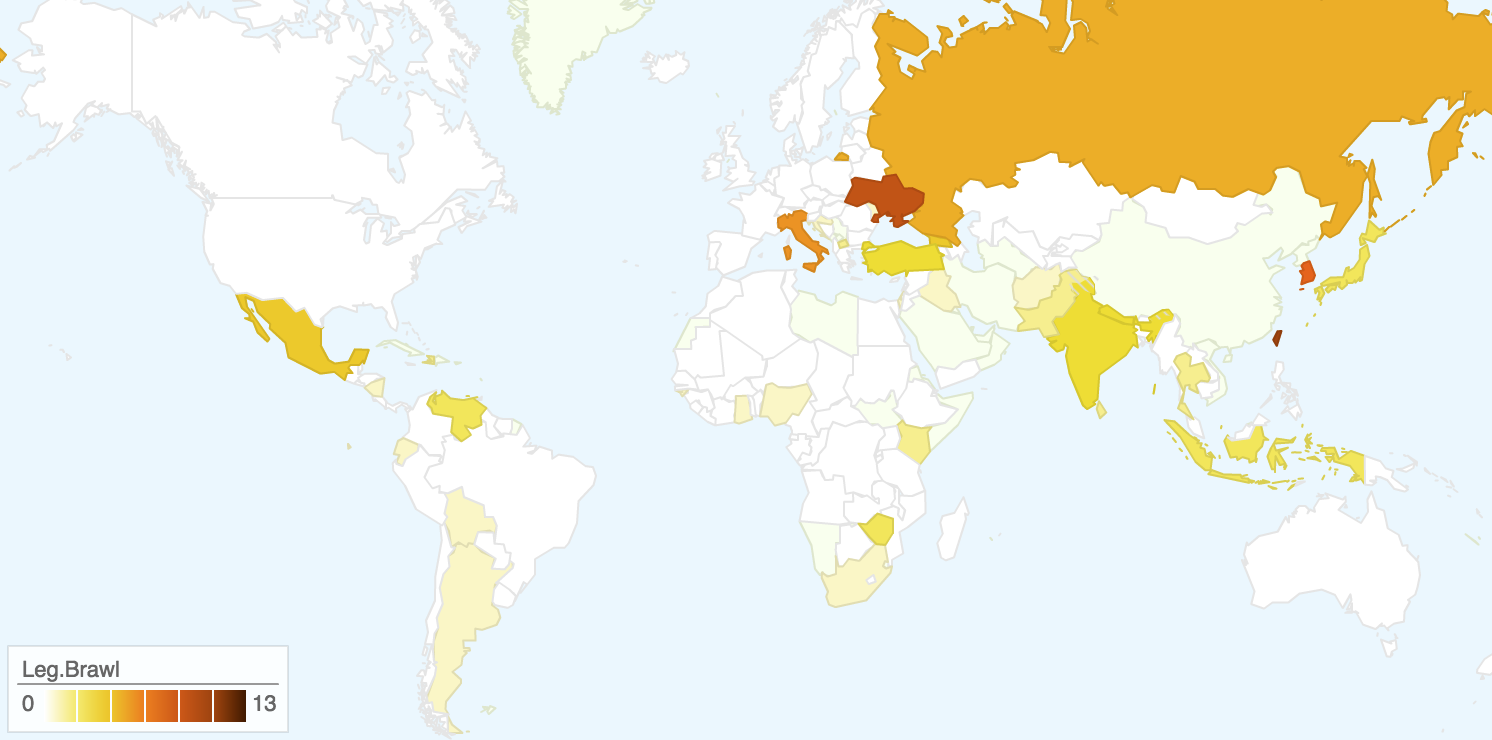
\includegraphics[width = 13cm]{incidence_map.png}

        \caption{\DIFaddFL{Incidences of Physical Fights Between Legislators in Democratic National Legislative Chambers (1981-2012)}}
        \label{leg_map}

\end{figure}

%DIF > %%%%%%%%%%%%%%% Scatterplot of Disproportionality, age_dem, and Violence %%%%%%%%%%%%%%%%%%%%%%%%
\begin{figure}[t]
    \begin{center}

\begin{knitrout}
\definecolor{shadecolor}{rgb}{0.969, 0.969, 0.969}\color{fgcolor}
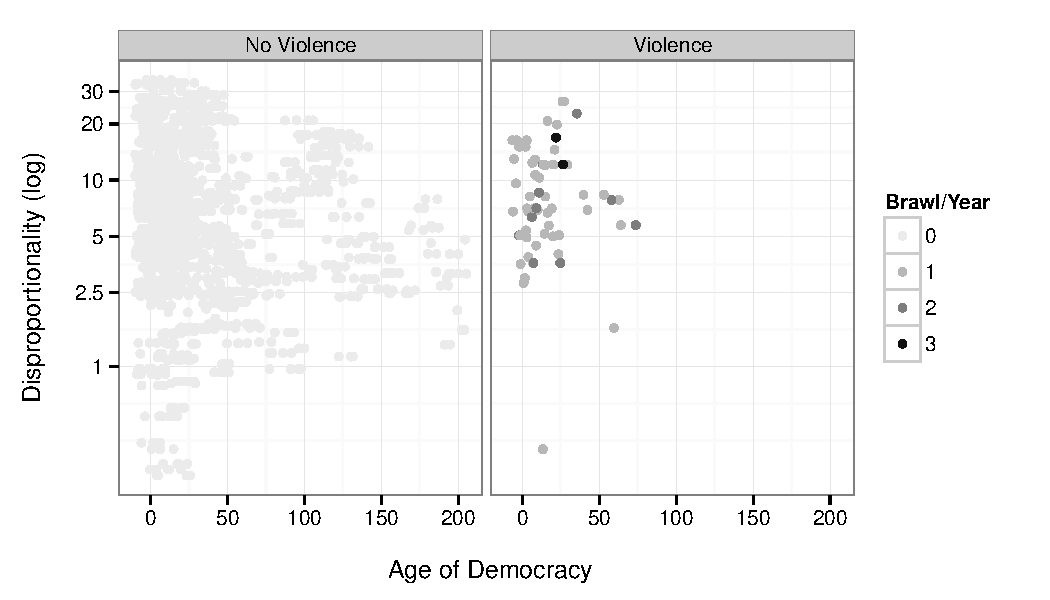
\includegraphics[width=0.8\linewidth]{figure/FrameworkEmpirical-1} 

\end{knitrout}
    \end{center}

    \caption{\DIFaddFL{Scatter plots of Disproportionality, Age of Democracy, and Violence in the Countries with }{\DIFaddFL{Elected Multi-party}}{\DIFaddFL{Democratic}} \DIFaddFL{National Legislatures.}}
    \label{framework_empirical}

    \begin{singlespace}
        {\scriptsize{Each point represents a country-year. The data is from a sample of countries from 1981 through 2012 due to data availability. The points are jittered horizontally.}}
    \end{singlespace}

\end{figure}

%DIF > %%%%%%%%%%%%%%% Run Analyses %%%%%%%%%%%%%%%%%%%%%%%%


%DIF > %%%%%%% Elected Legislatures Results Table from 1990
\begin{table}
\caption{\DIFaddFL{Legislative Violence Regression Results (Democratic Legislatures 1990-2012)}}
\label{outputTable.1990}
\begin{center}
\scalebox{0.8}{

% Table created by stargazer v.5.1 by Marek Hlavac, Harvard University. E-mail: hlavac at fas.harvard.edu
% Date and time: Tue, Apr 07, 2015 - 17:40:07
\begin{tabular}{@{\extracolsep{5pt}}lccccccc} 
\\[-1.8ex]\hline 
\hline \\[-1.8ex] 
 & \multicolumn{7}{c}{\textit{Dependent variable:}} \\ 
\cline{2-8} 
\\[-1.8ex] & \multicolumn{7}{c}{Violent Incident} \\ 
\\[-1.8ex] & (1) & (2) & (3) & (4) & (5) & (6) & (7)\\ 
\hline \\[-1.8ex] 
 Lower Disproportionality & $-$0.578$^{**}$ & $-$0.583$^{**}$ & $-$0.586$^{**}$ & $-$0.575$^{**}$ & $-$0.560$^{**}$ & $-$0.467 & $-$0.573$^{**}$ \\ 
  & (0.269) & (0.271) & (0.271) & (0.272) & (0.271) & (0.300) & (0.271) \\ 
  & & & & & & & \\ 
 Dem. Age (log) & $-$0.275$^{**}$ & $-$0.331$^{***}$ & $-$0.329$^{***}$ & $-$0.331$^{***}$ & $-$0.325$^{***}$ & $-$0.409$^{***}$ & $-$0.343$^{***}$ \\ 
  & (0.108) & (0.112) & (0.111) & (0.112) & (0.111) & (0.135) & (0.114) \\ 
  & & & & & & & \\ 
 Majority Size &  & $-$0.022$^{***}$ & $-$0.022$^{**}$ & $-$0.021$^{**}$ & $-$0.021$^{**}$ & $-$0.019$^{*}$ & $-$0.022$^{**}$ \\ 
  &  & (0.009) & (0.008) & (0.009) & (0.008) & (0.010) & (0.009) \\ 
  & & & & & & & \\ 
 Internal Armed Conflict &  &  & 0.440 & 0.421 & 0.413 & 0.386 & 0.449 \\ 
  &  &  & (0.344) & (0.347) & (0.344) & (0.386) & (0.345) \\ 
  & & & & & & & \\ 
 Leg. Immunity &  &  &  & 0.012 &  &  &  \\ 
  &  &  &  & (0.267) &  &  &  \\ 
  & & & & & & & \\ 
 Single Party Gov. &  &  &  & $-$0.049 &  &  &  \\ 
  &  &  &  & (0.263) &  &  &  \\ 
  & & & & & & & \\ 
 Political Constraints &  &  &  &  & $-$0.534 &  &  \\ 
  &  &  &  &  & (0.913) &  &  \\ 
  & & & & & & & \\ 
 Self Expression &  &  &  &  &  & 3.870 &  \\ 
  &  &  &  &  &  & (2.533) &  \\ 
  & & & & & & & \\ 
 Ethnic Frac. &  &  &  &  &  &  & $-$0.308 \\ 
  &  &  &  &  &  &  & (0.614) \\ 
  & & & & & & & \\ 
 (Intercept) & $-$2.120$^{***}$ & $-$0.735 & $-$0.807 & $-$0.811 & $-$0.671 & $-$5.675$^{*}$ & $-$0.659 \\ 
  & (0.307) & (0.559) & (0.561) & (0.655) & (0.625) & (3.180) & (0.645) \\ 
  & & & & & & & \\ 
\hline \\[-1.8ex] 
Observations & 1,492 & 1,441 & 1,441 & 1,419 & 1,417 & 810 & 1,435 \\ 
Log Likelihood & $-$260.703 & $-$254.213 & $-$253.577 & $-$252.777 & $-$252.611 & $-$188.719 & $-$253.279 \\ 
Akaike Inf. Crit. & 527.406 & 516.426 & 517.155 & 519.554 & 517.222 & 389.438 & 518.559 \\ 
\hline 
\hline \\[-1.8ex] 
\multicolumn{8}{l}{$^{*}$p$<$0.1; $^{**}$p$<$0.05; $^{***}$p$<$0.01} \\ 
\multicolumn{8}{l}{Standard errors are in parentheses. All models use robust (WEAVE) standard errors.} \\ 
\end{tabular} 

}
\end{center}
\end{table}


%DIF > %%%%%%%%%%%%%%% Expected Probability Graphs %%%%%%%%%%%%%%%%%%%%%%%%
\begin{figure}[t]
    \begin{center}

\begin{knitrout}
\definecolor{shadecolor}{rgb}{0.969, 0.969, 0.969}\color{fgcolor}
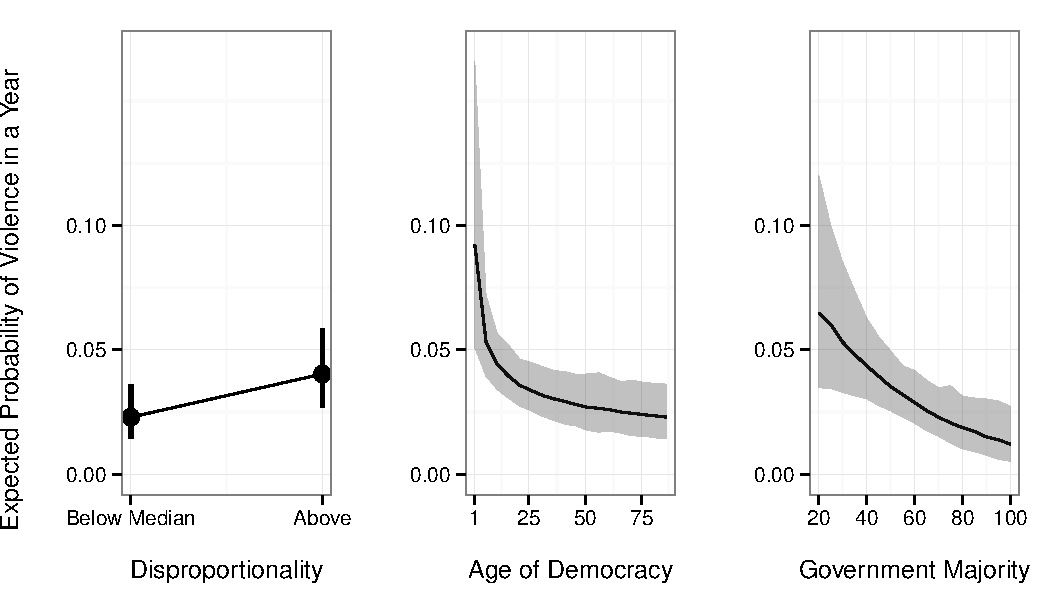
\includegraphics[width=0.95\linewidth]{figure/predProb-1} 

\end{knitrout}
    \end{center}
    \caption{\DIFaddFL{Expected Probability of Legislative Violence in Democratic Legislatures per Year}}
    \label{pred_prob}
    \begin{singlespace}
      {\scriptsize{The graphs show the median and middle 95\% of 1000 simulations at each fitted value of the variables. The simulations use estimates from Model 3, Table \ref{outputTable.1990}. For each set of simulations all other variables were fitted at their means.}}
    \end{singlespace}
\end{figure}
\DIFaddend 

\end{document}
